\documentclass[12pt,a4paper]{article}
\usepackage[a4paper, margin=0.6in]{geometry}
\usepackage[dvipsnames]{xcolor}
\usepackage[utf8]{inputenc}
\usepackage[T1]{fontenc} 
\usepackage[italian]{babel}
\usepackage{caption} %caption in minipage
%\selectlanguage{english}
\usepackage{amsmath,amsthm,amssymb,fge,mathrsfs}
%\usepackage{graphicx,txfonts}
\usepackage{mathtools}
\usepackage{centernot}
\usepackage{xfrac} %\for inline fractions
\usepackage{bbm}
\usepackage{menukeys}
\usepackage{listings}
\usepackage{pdfpages}
\usepackage{tikz-cd}
\usepackage{soul}
\usepackage[framemethod=TikZ]{mdframed}
\usepackage{dsfont}
\usepackage{pifont}% http://ctan.org/pkg/pifont
\usepackage{etoolbox}
\usepackage{hyperref}
\usepackage{mathabx}
\usepackage{makeidx} %per fare l'indice
\usepackage{faktor} %per i quozienti
%tikz (pacchetto per i disegni)
\usepackage{tikz}
\usetikzlibrary{arrows}
\usetikzlibrary{tikzmark}
\usetikzlibrary{calc} %per poter fare i calcoli
\usetikzlibrary{arrows.meta} %per usare veri tipi di frecce
\usetikzlibrary{calc,patterns,angles,quotes} %per disegnare gli angoli
\usetikzlibrary{decorations} %per i grafici orientati (con sopra le frecce)
%\usepackage{showlabels}
\usepackage{cases}
\usetikzlibrary{decorations.markings}
\usetikzlibrary{backgrounds} %per il colore sullo sfondo delle immagini
\usetikzlibrary{shapes.geometric} %per i triangoli negli alberi
\usetikzlibrary{patterns, positioning, arrows}
\usepackage{pgfplots}

\pgfplotsset{compat=newest}
\usepgfplotslibrary{fillbetween} %per colorare le aree comprese tra due grafici

%\usepackage{caption} %per la caption sotto alle immagini

\usepackage{tcolorbox}
\usepackage{cancel}
\tcbuselibrary{theorems}

%\newtcbtheorem[number within=section]{theorem}{Teorema}%
%{colback=green!5,colframe=green!35!black,fonttitle=\bfseries}{th}

\usepackage[tracking=true]{microtype} %per avvicinare il testo
\usepackage[shortlabels]{enumitem} %per modificare agilmente gli elenchi
\usepackage{esvect} %per le freccette di vettore sui caratteri
\usepackage{stmaryrd} %fulmine per il simbolo dell'assurdo
\usepackage{relsize} %per fare i simboli più grandi
\usepackage{mathabx} %per il simbolo di dotminus

\usepackage[customcolors]{hf-tikz} %per evidenziare pezzi di matrice

\usepackage{verbatim} %per commentare un blocco

\usepackage{multirow} %per la tabella
\usepackage{array} %per lo spazio nella tabella
\usepackage{empheq} % per sistema numerato

%Libreria per gli alberi
\usepackage[linguistics]{forest}

%Librerie aggiunte

%Libreria per i subfiles

\usepackage{subfiles} %meglio caricarla per ultima

\newtheorem{theorem}{Teorema}
\numberwithin{theorem}{section}
\newtheorem{corollary}[theorem]{Corollario}
\newtheorem{proposition}[theorem]{Proposizione}
\newtheorem{property}[theorem]{Proprieta}
\newtheorem{lemma}[theorem]{Lemma}

\newtheorem{definition}{Definizione}
\numberwithin{definition}{section}

\newtheorem*{remark}{Osservazione}

\newtheorem{example}{Esempio}
\numberwithin{example}{section}

\renewcommand*{\proofname}{dimostrazione}

%%%simboli speciali
\newcommand{\N}{\mathbb{N}}
\newcommand{\Z}{\mathbb{Z}}
\newcommand{\Q}{\mathbb{Q}}
\newcommand{\R}{\mathbb{R}}
\newcommand{\C}{\mathbb{C}}
\newcommand{\D}{\mathcal{D}}
\newcommand{\p}{\mathbb{P}}
\newcommand{\E}{\mathbb{E}}
\newcommand{\V}{\mathbb{V}ar}
\newcommand{\M}{\mathcal{M}}
\newcommand{\Hist}{\mathcal{H}}
\newcommand{\CO}{\mathcal{C}}
\newcommand{\F}{\mathbb{F}}
\newcommand{\G}{\mathcal{G}}
\newcommand{\Ecors}{\mathcal{E}}
\newcommand{\uno}{\mathbbm{1}}
\newcommand{\leb}{\mathcal{L}eb}
\newcommand{\lzu}{\mathcal{L}eb_{(0,1)}}
\newcommand{\TCM}{\color{orange} \bf{TCM } \color{black}}
\newcommand{\SSI}{\color{orange} \bf{SSI } \color{black}}
\newcommand{\TCD}{\color{PineGreen} \bf{TCD } \color{black}}
\newcommand{\TRN}{\color{red} \bf{Teorema di Radon-Nikodym } \color{black}}
\newcommand{\Dambro}{\color{orange} \bf{Caratterizzazione delle funzioni positive con funzioni semplici, sotto il segno di D'Ambrosio }\color{black}}



\newcommand\incorr{\protect\mathpalette{\protect\independenT}{\perp}}
\def\independenT#1#2{\mathrel{\rlap{$#1#2$}\mkern2mu{#1#2}}}
\newcommand{\soprasotto}[3]{\ensuremath\underset{\text{#2}}{\overset{\text{ #1}}{#3}}}
\def\salg{\ensuremath\sigma \text{-algebra }}
\def\salge{\ensuremath\sigma \text{-algebre }}
\newcommand{\tc}{\ \lvert \ }
\newcommand{\Rbar}{\overline{\mathbb{R}}}
\newcommand{\Xbar}{\overline{X}}

\newcommand{\cmark}{\Large\color{green}\ding{51}\color{black}\normalsize}%
\newcommand{\xmark}{\Large\color{red}\ding{55}\color{black}\normalsize}%

\newcommand{\Bo}[1]{\mathcal{B}(#1)}

\newcommand{\deftitle}[1]{{\color{red}\bf{#1}\color{black}}}
\newcommand{\dftitle}[2]{{\color{#2}\bf{#1}\color{black}}}
\newcommand{\cuore}[1]{\Large\color{#1}\ding{170}\color{black}\normalsize}

\newcommand{\toxic}{\deftitle{Toxic Relationship fra $\sigma X$ e $f(X)$ }}

\newcommand{\x}{ \textit{\textbf x}}
\newcommand{\cc}{ \textit{\textbf c}}
\newcommand{\vcors}{ \textit{\textbf v}}
\newcommand{\ww}{ \textit{\textbf w}}

\newcommand{\triangolino}{\ensuremath\scriptscriptstyle {\triangle}}

\newcommand{\ser}{\sum\limits_{n=0}^\infty}








\newcounter{theo}[section]\setcounter{theo}{0}
\renewcommand{\thetheo}{\arabic{section}.\arabic{theo}}
\newenvironment{theo}[2][]{%
	\refstepcounter{theo}
	
	\ifstrempty{#1}%
	% if condition (without title)
	{\mdfsetup{%
			frametitle={%
				\tikz[baseline=(current bounding box.east),outer sep=0pt]
				\node[anchor=east,rectangle,fill=cyan!10]
				{\strut Teorema~\thetheo};}
		}%
		% else condition (with title)
	}{\mdfsetup{%
			frametitle={%
				\tikz[baseline=(current bounding box.east),outer sep=0pt]
				\node[anchor=east,rectangle,fill=cyan!10]
				{\strut Teorema~\thetheo:~#1};}%
		}%
	}
	% Both conditions
	\mdfsetup{%
		innertopmargin=10pt,linecolor=cyan!20,%
		linewidth=2pt,topline=true,%
		frametitleaboveskip=\dimexpr-\ht\strutbox\relax%
	}
	
	\begin{mdframed}[]\relax}{%
\end{mdframed}}

\newcounter{eser}[section]\setcounter{eser}{0}
\renewcommand{\theeser}{\arabic{section}.\arabic{eser}}
\newenvironment{eser}[2][]{%
	\refstepcounter{eser}
	
	\ifstrempty{#1}%
	% if condition (without title)
	{\mdfsetup{%
			frametitle={%
				\tikz[baseline=(current bounding box.east),outer sep=0pt]
				\node[anchor=east,rectangle,fill=cyan!10]
				{\strut Esempio~\theeser};}
		}%
		% else condition (with title)
	}{\mdfsetup{%
			frametitle={%
				\tikz[baseline=(current bounding box.east),outer sep=0pt]
				\node[anchor=east,rectangle,fill=cyan!10]
				{\strut Esempio~\theeser:~#1};}%
		}%
	}
	% Both conditions
	\mdfsetup{%
		innertopmargin=10pt,linecolor=cyan!20,%
		linewidth=2pt,topline=true,%
		frametitleaboveskip=\dimexpr-\ht\strutbox\relax%
	}
	
	\begin{mdframed}[]\relax}{%
\end{mdframed}}

\newcounter{lem}[section]\setcounter{lem}{0}
\renewcommand{\thelem}{\arabic{section}.\arabic{lem}}
\newenvironment{lem}[2][]{%
	\refstepcounter{lem}
	
	\ifstrempty{#1}%
	% if condition (without title)
	{\mdfsetup{%
			frametitle={%
				\tikz[baseline=(current bounding box.east),outer sep=0pt]
				\node[anchor=east,rectangle,fill=Melon!20]
				{\strut Lemma~\thelem};}
		}%
		% else condition (with title)
	}{\mdfsetup{%
			frametitle={%
				\tikz[baseline=(current bounding box.east),outer sep=0pt]
				\node[anchor=east,rectangle,fill=Melon!20]
				{\strut Lemma~\thelem:~#1};}%
		}%
	}
	% Both conditions
	\mdfsetup{%
		innertopmargin=10pt,linecolor=Melon!20,%
		linewidth=2pt,topline=true,%
		frametitleaboveskip=\dimexpr-\ht\strutbox\relax%
	}
	
	\begin{mdframed}[]\relax}{%
\end{mdframed}}



\newcounter{prf}[section]\setcounter{prf}{0}
\renewcommand{\theprf}{\arabic{section}.\arabic{prf}}
\newenvironment{prf}[2][]{%
	\refstepcounter{prf}%
	\ifstrempty{#1}%
	{\mdfsetup{%
			frametitle={%
				\tikz[baseline=(current bounding box.east),outer sep=0pt]
				\node[anchor=east,rectangle,fill=red!20]
				{\strut Dimostrazione~\theprf};}}
	}%
	{\mdfsetup{%
			frametitle={%
				\tikz[baseline=(current bounding box.east),outer sep=0pt]
				\node[anchor=east,rectangle,fill=red!20]
				{\strut Dimostrazione~\theprf:~#1};}}%
	}%
	\mdfsetup{innertopmargin=10pt,linecolor=red!20,%
		linewidth=2pt,topline=true,%
		frametitleaboveskip=\dimexpr-\ht\strutbox\relax
	}
	\begin{mdframed}[]\relax%
		\label{#2}}{\end{mdframed}}


\newcounter{defi}[section]\setcounter{defi}{0}
\renewcommand{\thedefi}{\arabic{section}.\arabic{defi}}
\newenvironment{defi}[2][]{%
	\refstepcounter{defi}
	
	\ifstrempty{#1}%
	%	% if condition (without title)
	{\mdfsetup{%
			frametitle={%
				\tikz[baseline=(current bounding box.east),outer sep=0pt]
				\node[anchor=east,rectangle,fill=green!20]
				{\strut Definizione~\thedefi};}
		}%
		% else condition (with title)
	}{\mdfsetup{%
			frametitle={%
				\tikz[baseline=(current bounding box.east),outer sep=0pt]
				\node[anchor=east,rectangle,fill=green!20]
				{\strut Definizione~\thedefi:~#1};}%
		}%
	}
	% Both conditions
	\mdfsetup{%
		innertopmargin=10pt,linecolor=green!20,%
		linewidth=2pt,topline=true,%
		frametitleaboveskip=\dimexpr-\ht\strutbox\relax%
	}
	
	\begin{mdframed}[]\relax}{%
\end{mdframed}}








%%%%%%%%%%%%%%%%%%%%%%%%%%%%%%%%%%%%%%%%%%%%%%%%%%%%%%%%%%%%%%%%%%%%%%%%%%%%%%%%%%%%%%%%%%%%%%%%%%%%%%%%%%%%%%%%%%%%%%%%%%%%%%%%%%%%%%%%%%%%%%%%%%%%%%%%%%%%%%%%%%%%%%%%%%%%%%%%%%%%%%%%%%%%%%%%%%%%%%%%%%%%%%%%%%%%%%%%%%%%%%%%%%%%%%%%%%%%%%%%%%%%%%%%%%%%%%%%%%%%%%%%%%%%%%%%%%%%%%%%%%%%%%%%%%%%%%%%%%%%%%%%%%%%%%%%%%%%%%%%%%%%%%%%%%
\newcommand{\palla}{
	\begin{tikzpicture}
		\node[circle,fill=red!60!RawSienna,inner sep=2pt, scale=2] { };
	\end{tikzpicture}
}

\newcommand{\ball}[1]{
	\begin{tikzpicture}
		\node[circle,fill=#1,inner sep=2pt, scale=2] { };
	\end{tikzpicture}
}

\newcommand{\balln}[2]{
	\begin{tikzpicture}
		\node[circle,fill=#1,inner sep=2pt, scale=1] {#2};
	\end{tikzpicture}
}


\DeclareMathOperator{\Ima}{Im}

\DeclareMathOperator{\mcd}{MCD}
\DeclareMathOperator{\mcm}{mcm}

\DeclarePairedDelimiter\abs{\lvert}{\rvert}
\DeclarePairedDelimiter\norm{\lVert}{\rVert}

%Necessario per far si che la dimensione del valore assoluto e della norma si adatti all'aromento passato
\makeatletter
\let\oldabs\abs
\def\abs{\@ifstar{\oldabs}{\oldabs*}}
%
\let\oldnorm\norm
\def\norm{\@ifstar{\oldnorm}{\oldnorm*}}
\makeatother

%Spaziatura per i quantificatori
\let\oldforall\forall
\renewcommand{\forall}{\; \oldforall \;}
\let\oldexists\exists
\renewcommand{\exists}{\; \oldexists \;}



%%%%%%%%%%%%%%%%%%%%%%%%%%%%%%%%%%%%%%%%%%%%%%%%%%%%%%%%%%%%%%%%%%%%%%%%%%%%%%%%%%%%%%%%%%%%%%%%%%%%%%%%%%%%%%%%%%%%%%%%%%%%%%%%%%%%%%%%%%%%%%%%%%%%%%%%%%%%%%%%%%%%%%%%%%%%%%%%%%%%%%%%%%%%%%%%%%

\title{Il Gambero della Louisiana nel Parco delle Alpi Marittime}
\author{Matteo Bracco, Cecilia Zannotti, Marco Lugarà}
\date{30 maggio 2024}

\begin{document}
\maketitle
\section{E-mail}
Email dei partecipanti
	\begin{itemize}[\palla]
		\item Matteo Bracco: matteo.bracco198@edu.unito.it
		\item Cecilia Zannotti: cecilia.zannotti@edu.unito.it
		\item Marco Lugarà: marco.lugara@edu.unito.it
	\end{itemize}
\section{Problematica}
Il Gambero della Lousiana, \textit{Procamburus Clarkii}, è stato introdotto in Italia tramite acquacultura. La specie è particolarmente edace e distruttrice, si adatta bene a quasi tutti i contesti di acqua dolce o salmastra\cite{mase.gov}. Le principali problematiche relative alla loro presenza sono
\begin{itemize}[\palla]
	\item Diffusione di malattie, in particolare la peste del gambero (\textit{Aphanomyces astaci}) nelle specie di gambero d'acqua dolce autoctone dell'Italia, come \textit{Austropotamobius pallipes italicus}, già minacciate da altri fattori fra i quali l'inquinamento delle acque. La diffusione non avviene per contatto diretto fra gamberi; il gambero autoctono viene infettato dalle spore del fungo, che possono essere trasportate tramite attrezzatura da pesca per esempio, oppure dal gambero della Louisiana, che possiamo considerare come portatore sano della malattia.
	\item È un animale onnivoro estremamente vorace, si ciba di uova, avanotti, piccoli anfibi, per esempio nel Parco del delta del Po ha causato l'estinzione del $45\%$ delle specie di Odonati (insetti simili alle libellule) \cite{lifeclaw}. Studiando il fenomeno all'interno del Parco delle Alpi Marittime, potrebbe essere interessante la relazione con specie endemiche come lo Scazzone, %(pesciolino) 
    nel caso possano esistere dei pericoli.
	\item Produce anche danni economici, per esempio mangia i germogli nelle risaie; danni geologici, per lo scavo degli argini in cui crea le sue tane; inoltre è ospite di parassiti intermedi pericolosi per uomini e animali da compagnia.
\end{itemize}


\section{Possibili Azioni}
Al fine di inquadrare al meglio la situazione ed avere un parere diretto sul fenomeno, abbiamo contattato il Parco delle Alpi Marittime e ci siamo fatti spiegare meglio quali sono i pericoli attuali e quali possono essere le modalità per affrontarli.

Per il momento, il Parco ha solamente iniziato un'attività volta a monitorare la presenza di questo gambero nelle sue acque, sarebbe interessante analizzare alcune tecniche volte all'eliminazione della specie, come previsto dal Piano Nazionale \cite{mase.gov}. Alcune azioni possono essere: introdurre esemplari di maschi sterili insieme ad una cattura intensiva tramite nasse, volta a limitare la densità di popolazione, oppure aumentare i predatori indigeni (uccelli, trote), \cite{lifeclawazioni}, \cite{mase.gov}.

\bigskip
Date le precedenti considerazioni, elenchiamo di seguito alcune popolazioni che potrebbero essere analizzate nel modello.
\begin{itemize}[\palla]
	\item Gambero della Louisiana \textit{Procamburus Clarkii} $L$
	\item IL Gambero d'acqua dolce \textit{Austropotamobius pallipes italicus} $G$.
	\item La Peste del gambero, \textit{Aphanomyces astaci}, eventualmente separando spore $Z$ dai funghi sul gambero $F$
	\item Possibili prede (Scazzone, Odonati) $S$
	\item Possibili predatori (Trote o Uccelli).
\end{itemize}
%\textit{Nota} Alcune specie possono predarsi a vicenda: ad esempio gli avanotti (piccole trote), possono essere mangiate dai gamberi, che viceversa sono predati da trote di dimensione maggiore.


\section{Primo Modello}
Abbiamo deciso di analizzare la sopravvivenza del Gambero autoctono in presenza del Gambero della Louisiana e della Peste del gambero; ci concentriamo quindi sull'interazione tra le due specie di gambero e la diffusione della malattia, mentre le prede comuni e i predatori di gamberi non compariranno direttamente all'interno del modello, per contenere il numero di popolazioni.

Dunque consideriamo, in partenza, cinque popolazioni per un primo modello:
\begin{itemize}[\palla]
    \item Zoospore del fungo $Z$
	\item Il Fungo Peste del gambero allo stato riproduttivo $F$
	\item Gamberi della Louisiana totali $L$
	\item Gamberi delle Louisiana infetti $I$
	\item Gamberi Autoctoni $G$
\end{itemize}
\begin{itemize}
	\item[\dftitle{$Z$}{cyan}] Il Fungo adulto $F$ produce in media $c_1$ spore. Le spore nell'acqua muoiono con un rate $m_1$, inoltre vi sono i termini di migrazione quando avviene l'infezione delle Zoospore $Z$.
	\item[\dftitle{$F$}{cyan}] la variazione dei Funghi adulti $F$ è proporzionale alla popolazione di Gamberi della Louisiana infetti, dove $c_2$ rappresenta il numero medio di Funghi per individuo infetto, inoltre diminuisce con rate $m_2$.
	\item[\dftitle{$L$}{cyan}] Dato che non risente della malattia, la variazione della popolazione dei Gamberi della Louisiana, ha due componenti, una demografica e una di competizione con il gambero nostrano $G$ determinata dal coefficiente $a_2$. 
    \item[\dftitle{$I$}{cyan}] I gamberi della Louisiana si infettano a causa dell'incontro con Zoospore $Z$ nell'ambiente, con un tasso $\gamma_2$, ma poichè non risentono della malattia hanno un tasso di mortalità pari a quello dei Gamberi della Louisiana totali $L$.
    \item[\dftitle{$G$}{cyan}] I gamberi nostrani muoiono non appena contraggono la malattia, inoltre vi è competizione con $L$, determinata dal coefficiente $a_1$, e infine la parte demografica, che segue il modello logistico.
\end{itemize} 
\textit{Nota} La competizione tra i due gamberi è molto a sfavore del gambero autoctono. Nella realtà, quindi, molto probabilmente si avrà che $a_1 > a_2$.
%Usa i commenti
$$\begin{cases*}
    \dot Z= c_1F-m_1 Z -\gamma_2LZ-\gamma_1GZ  \\
	\dot F= c_2I - m_2 F  \\
     \dot G= -\gamma_1  GZ - a_1GL +b_1 G - m_3 G^2 \\
	\dot L=  -a_2 GL+b_2 L - m_4 L^2 \\
	\dot I=\gamma_2 LZ-m_4 I \\
\end{cases*}$$
Analizziamo i vari pezzi di ogni equazione: \\
\dftitle{Equazione $1$}{blue}
\begin{itemize}[\palla]
    \item $c_1 F$: incremento di spore, dovuto alla produzione dei funghi
    \item $-m_1 Z$: diminuizione delle spore, relativo al tasso di mortalità $m_1$
    \item $-\gamma_1 GZ$: diminuzione delle spore dovute all'infezione di $G$, passano nella popolazione di $F$
    \item $-\gamma_2 LZ$: diminuzione delle spore dovute all'infezione di $L$, passano nella popolazione di $F$
\end{itemize}
\dftitle{Equazione $2$}{blue}
\begin{itemize}[\palla]
    \item $c_2 I$: incremento di funghi proporzionale al numero di gamberi infetti $I$
    \item $-m_2 F$: diminuizione dei funghi, rispetto al tasso di mortalità $m_2$
\end{itemize}
\dftitle{Equazione $3$}{blue}
\begin{itemize}[\palla]
    \item $-a_2 GL$: diminuzione di $L$ dovuta alla competizione con $G$
    \item  $b_2L-m_4 L^2$: modello di crescita logistica per $L$, notare che la capacità portante è data da $\frac{b_2}{m_4}$
\end{itemize} 
\dftitle{Equazione $4$}{blue}
\begin{itemize}[\palla]
    \item  $\gamma_2 LZ$: incremento degli infetti nella popolazione di $L$ 
\item  $-m_4 I$: diminuzione  dei gamberi infetti, rispetto al tasso di mortalità $m_4$ condiviso con la popolazione totale $L$ 
\end{itemize}
\dftitle{Equazione $5$}{blue}
\begin{itemize}[\palla]
    \item $-\gamma_1 GZ$: morte istantanea nei gamberi $G$, dovuta all'infezione
    \item $-a_1 GL$: diminuzione  di $G$ dovuta alla competizione con $L$
\item  $b_1 G-m_3G^2$: modello logistico per $G$ con capacità portante $\frac{b_1}{m_3}$

\end{itemize} 


%. Invece, le zoospore possono diventare "adulte" sia sui gamberi nostrani sia su quelli invasivi, nel secondo caso però portano alla morte. Dovremmo teoricamente considerare due coefficienti diversi $\beta_1,\beta_2$ che portano alla maturazione delle spore all'interno dei gamberi, ma qua possono essere molto simili infondo, ed essere presi uguali se i parametri diventano troppi. Invece, le zoospore riescono a maturare anche su altre superifici (quali pesci o rocce), senza causare danni ma producendo altre zoospore, anche se meno efficacemente e per un numero limitato di volte (tipo $3$, questo però l'abbiamo trovato solo in un articolo), il che potrebbe essere assorbito considerando un $\Lambda$ diverso nella sopravvivenza fuori dall'acqua. I funghi adulti all'interno dei gamberi sopravvivono producendo spore, sembrerebbe che nei gamberi invasivi ne producano di più, e che il fungo si riproduca più velocemente. Il che significa che $c_1>c_2$ dove $c_i$ rappresenta la quantità di spore prodotte da un fungo all'interno del suo host. Forse dovremmo mettere qualcosa che conta la rapidità di crescita, ma si può riflettere interpretando meglio i $c_i$. La mortalità sul gambero nostrano è praticamente del $100\%$, quindi possiamo non mettere il rate di mortalità, dobbiamo però inserire $\lambda=\frac 1 {T'}$ 
%

%
%%PLEASE ALMENO TOGLIAMO Z
%
%%Per quanto riguarda la malattia, possiamo fare riferimento a
%%\textit{"Sono fonti di contagio i gamberi infetti e morti nonché quelli non autoctoni portatori della malattia benché non affetti. La trasmissione può avvenire anche tramite pesci provenienti da zone contaminate o apparecchiature infette (stivali, abiti, reti, ecc.)."} \cite{fungo}

%Per il gambero autoctono, con un certo rate $\gamma$ dall'incontro con un gambero della Louisiana o di un altro gambero autoctono si produce un contagio che con un rate $\beta_2$ porta alla morte. Quindi posto $\beta=\beta_1\cdot\beta_2$, il termine d'interazione sarà dato da $-\beta (P+S) S$.Inoltre il gambero può morire anche dall'interazione con l'ambiente, in quanto può contrarre la malattia (nell'ambiente ci mettiamo anche i gamberi morti), o morire a causa dell'inquinamento, riassumiamo il tutto in un coefficiente $\mu$ di mortalità. Infine, mettiamo un termine di crescita dovuto all'interazione con le prede, il cui rate è $\gamma$; ed una crescita logistica dovuta alla presenza di cibo alternativo e risorse limitate, molto probabile, tipo uova di altri pesci, e materiale organico fresco (dobbiamo controllare che si mangino anche le prede $Z$) $\lambda$. (Abbiamo controllato è abbastanza credibile vedi \cite{cibo})
%$$\dot S= -\beta (P+S) S-\mu_1 S +\gamma_1 S Z+\lambda_1 S(1-S)$$
%
%Per quanto riguarda invece il gambero della Louisiana, esso è soltanto portatore della malattia, ma non è affetto da essa. Quindi non muore per l'incontro con altri gamberi, esso quindi presenterà solamente i termini con $\mu_2,\gamma_2,\lambda_2$ dove $\mu_2 << \mu_1$ vista che non è affetto da malattia\cite{fungo} e non è suscettibile all'inquinamento \cite{articoloparco}, $\gamma_2 >> \gamma_1$ per la voracità del gambero della Louisiana, e probabilmente quindi pure $\lambda_2>\lambda_1$. Nel coeffiienti $\mu_i$ vanno anche considerati i termini di predazione di eventuali uccelli/trote. In un secondo momento, invece, studiamo come l'introduzione di maschi sterili di gamberi della Louisiana nell'ambiente \cite{articolo_parco}, che supponiamo impattare effettivamente sui coefficienti $\gamma_2,\lambda_2$ in modo da ridurli drasticamente, modifichi il modello.
%
%$$\dot P= -\mu_2 P +\gamma_2 P Z+\lambda_2 P(1-P)$$
%
%Infine per le prede, supponiamo una crescita logistica data dal coefficiente $\lambda_3$ e la predazione congiunta delle due specie di gamberi
%
%\[
%\dot Z=\lambda_3 Z(1-Z)-\gamma_2 -PZ-\gamma_1 SZ
%\]

\bigskip

Ci rendiamo però conto che con questo modello quando un individuo di $L$ viene infettato passa in $I$, allora correggiamo l'errore come segue

$$\begin{cases*}
	\dot Z= c_1F-m_1 Z -\gamma_2LZ-\gamma_1GZ \\
	\dot F= c_2I - m_2 F \\
  \dot G= -\gamma_1  GZ - a_1GL +b_1 G - m_3 G^2 \\
	\dot L=  -a_2 GL+b_2 L - m_4{L^2}-\deftitle{\gamma_2 LZ} \\ %ma perchè?
	\dot I=\gamma_2 LZ-m_4 I \\	
\end{cases*}$$

Tuttavia qualcosa continua ad essere errato dato che, in realtà, $L$ ed $I$ non sono popolazioni completamente diverse, sono piuttosto una la sottopopolazione dell'altra e la loro variazione è essenzialmente la stessa.


\section{Secondo Modello}
Riteniamo dunque che sia opportuno rimuovere $I$ dal modello e consideriamo che i Funghi $F$ varino al variare delle infezioni del Gambero della Louisiana $L$. Il nuovo modello sarà allora il seguente

$$\begin{cases*}
	\dot Z= c_1F-m_1 Z -\gamma_2 LZ-\gamma_1GZ \\
	\dot F= c_2 \gamma_2LZ  - m_2 F \\
	\dot G= -\gamma_1 GZ - a_1 LG+b_1 G -m_3 G^2 \\
	\dot L=  -a_2LG+b_2 L -m_4 L^2 
\end{cases*}$$

\smallskip
In particolare il pezzo $c_2 \gamma_2LZ  - m_2 F$ spiega che $F$ varia con il numero di infezioni, dove $c_2$ è il numero medio di funghi per infezione. \\
Inoltre osserviamo che nell'equazione di $L$ non c'è più il pezzo $-\gamma_2 LZ$, in quanto abbiamo eliminato la variabile $I$. \\
Infine decidiamo di inserire un termine di sopravvivenza del Fungo anche sui Gamberi di acqua dolce, cioè il Fungo continua a vivere e produrre spore per un periodo breve (quantificato da $\lambda$ piccolo) anche se il Gambero è già morto, \cite{strand2012monitoring}, \cite{makkonen2013timing}: $c_2 \lambda \gamma_1 GZ$. \\
Inoltre ci accorgiamo, dai conti, che manca un termine di interazione intraspecifica per le Zoospore: $a_3 Z^2$.

$$\begin{cases*}
    \dot Z= c_1F-m_1 Z -\gamma_2 LZ-\gamma_1GZ - \deftitle{a_3 Z^2}  \\
    \dot F= c_2(\gamma_2LZ  + \deftitle{\lambda \gamma_1 GZ})- m_2 F \\
    \dot G= -\gamma_1 GZ - a_1 LG+b_1 G -m_3 G^2 \\
    \dot L= -a_2LG+b_2 L -m_4 L^2
\end{cases*}$$

\medskip
Riassumendo, i termini differenti dal modello precedente: \\
\dftitle{Equazione $1$}{blue}
\begin{itemize}[\palla]
    \item $c_1 F$: incremento di spore, dovuto alla produzione dei funghi
    \item $-m_1 Z$: diminuizione delle spore, relativo al tasso di mortalità $m_1$
    \item $-\gamma_1 GZ$: diminuzione delle spore dovute all'infezione di $G$, passano nella popolazione di $F$
    \item $-\gamma_2 LZ$: diminuzione delle spore dovute all'infezione di $L$, passano nella popolazione di $F$
    \item $-a_3 Z^2$: diminuzione delle spore per interazione interspecifica con tasso $a_3$
\end{itemize}
\dftitle{Equazione $2$}{blue}
\begin{itemize}[\palla]
    \item $c_2 \gamma_2LZ$: variazione di $F$ dovuta alla infezione di gamberi $L$, dove $c_2$ è il numero medio di funghi prodotti per infezione
    \item $c_2 \lambda \gamma_1 GZ$: variazione di $F$ dovuta alla sopravvivenza del fungo, per un breve periodo indicato da $\lambda$, su gamberi $G$ morti a seguito dell'infezione, dove $c_2$ è il numero medio di funghi prodotti per infezione
    \item  $-m_2 F$: variazione istantanea di $F$ dovuta alla morte dei funghi
\end{itemize}

%\bigskip
\newpage
\begin{center}
\textbf{MODELLO FINALE}
\begin{numcases}{}
    & $\dot Z= c_1F-m_1 Z -\gamma_2 LZ-\gamma_1GZ - a_3 Z^2$  \\
    & $\dot F= c_2(\gamma_2LZ  + \lambda \gamma_1 GZ)- m_2 F$ \\
    & $\dot G= -\gamma_1 GZ - a_1 LG+b_1 G -m_3 G^2$ \\
    & $\dot L= -a_2LG+b_2 L -m_4 L^2$
\end{numcases}
\end{center}

\medskip

\dftitle{Tabellina riassuntiva per i Parametri}{blue}
\begin{itemize}[\palla]
    \item $a_1 =$ competizione interspecifica $L,G$ di cui risente $G$
    \item $a_2 =$ competizione interspecifica $L,G$ di cui risente $F$
    \item $a_3 =$ fattore di competizione intraspecifico di $Z$
    \item $b_1 =$ tasso di crescita di $G$
    \item $b_2 =$ tasso di crescita di $L$
    \item $c_1 =$ numero medio di spore $Z$ prodotte da un fungo $F$
    \item $c_2 =$ numero medio di funghi 
$F$ prodotti per ogni infezione
    \item $m_1 =$ tasso di mortalità di $Z$
    \item $m_2 =$ tasso di mortalità di $F$
    \item $m_3 =$ fattore di competizione\footnote{corrisponde al rapporto fra rate di crescita e capacità portante per $G$}intraspecifica per $G$
    \item $m_4 =$ fattore di competizione\footnote{corrisponde al rapporto fra rate di crescita e capacità portante per $L$} intraspecifica per $L$
    \item $\lambda =$ fattore che tiene conto della sopravvivenza  del fungo $F$ sulle carcasse del gambero $G$
    \item $\gamma_1 =$ tasso di infezione delle spore $Z$ sul gambero $G$
    \item $\gamma_2 =$ tasso di infezione delle spore $Z$ sul gambero $L$
\end{itemize}


\newpage


\section{Equilibri e Ammisibilità}

Analizziamo gli Equilibri di questo modello. Di seguito la Tabella Binaria, Tabella \ref{tab:equilibri}.
\begin{table}[h]
	\begin{tabular}{|c|c|c|c|c|c|c|}
		\hline
		\textbf{Z} & \textbf{F}& \textbf{G} & \textbf{L} &  & &  \\
		\hline
		0 & 0 & 0 & 0 & \cmark &  $E_0=(0,0,0,0)$ & \\
		\hline
		0 & 0 & 0 & 1 & \cmark & $ E_1=(0,0,0,\frac{b_2}{m_4})$ & $b_2L-m_4L^2=0 \implies L_1= \frac{b_2}{m_4} $ \\
		\hline
		0 & 0 & 1 & 0 & \cmark & $E_2=(0,0,\frac{b_1}{m_3},0)$ & $b_1G-m_3G^2=0 \implies G_2= \frac{b_1}{m_3} $ \\
  		\hline
		0 & 0 & 1 & 1 & $\text{\cmark}^\ast$ & $E_3$ &  dettagli dopo la tabella \\
		\hline
		0 & 1 & 0 & 0 & \xmark & Eq 2 (F) & $ -m_2F=0 $ \\
  		\hline
		0 & 1 & 0 & 1 & \xmark & Eq 2 (F) &  $ -m_2F=0 $ \\
  		\hline
		0 & 1 & 1 & 0 & \xmark & Eq 2 (F) &  $ -m_2F=0 $ \\
  		\hline
		0 & 1 & 1 & 1 & \xmark & Eq 1 (Z)  & $ c_1 F=0 $ \\





  
		\hline
		1 & 0 & 0 & 0 & \xmark & Eq 1 (Z)  & $ -m_1Z-a_3Z^2=0\implies Z=-\frac{m_1}{a_3}$  non ammissibile\\
		\hline
		1 & 0 & 0 & 1 & \xmark & Eq 2 (F) & $  c_2\gamma_2LZ=0 \implies L=0 \vee Z=0$ \\
  		\hline
		1 & 0 & 1 & 0 & \xmark & Eq 2 (F) & $  c_2\lambda \gamma_1 GZ=0 \implies G=0 \vee Z=0$ \\
  		\hline
		1 & 0 & 1 & 1 & \xmark & Eq 2 (F) &  $ c_2(\gamma_2 LZ+\lambda \gamma_1 GZ)=0 \implies Z=0 \vee L=-\frac{\lambda\gamma_1}{\gamma_2} G$ \\
		\hline
		1 & 1 & 0 & 0 & \xmark & Eq 2 (F) & $ -m_2F=0 $ \\

	\hline
	1 & 1 & 0 & 1 &  $\text{\cmark}^\ast$ &$E_5$ &  dettagli dopo la tabella \\
	\hline
	1 & 1 & 1 & 0 &  $\text{\cmark}^\ast$ & $E_4$ &  dettagli dopo la tabella \\
	\hline
	1 & 1 & 1 & 1 &  $\text{\cmark}^\ast$ & $E_6$ &  dettagli dopo la tabella \\
		\hline
	\end{tabular}
 \caption{Tabella Binaria}
 \label{tab:equilibri}
\end{table}

%\newpage
\vspace{1 cm}

Vediamo a parte le condizione di ammissibilità per gli equilibri $E_3,E_4,E_5,E_6$.

\begin{itemize}
	\item[\balln{yellow}{$E_3$}]
	Qui abbiamo $Z=F=0$. Il sistema diventa
	$$\begin{cases*}
		\dot Z=0 \\
		\dot F=0 \\
		\dot G=-a_1 L G+b_1 G-m_3 G^2=0 \\
		\dot L=-a_2 LG+b_2 L-m_4 L^2=0
	\end{cases*}$$
Ci si riduce quindi ad un modello di competizione intraspecifica fra le due specie di gamberi. Semplificando $L$ e $G$ nelle due equazioni, risolvendo per $G$ e sostituendo nella quarta equazione ($\dot L=0$) quanto trovato, otteniamo
\[\begin{cases*}
	G_3=\frac{b_1-a_1 L_3}{m_3} \\
	-a_2 \frac{b_1-a_1 L_3}{m_3}+b_2 -m_4 L_3=0
\end{cases*}
\] 
Possiamo allora ricavare $L_3$ e poi $G_3$ sostituendo a ritroso. Posto $D=a_2a_1-m_4m_3$ si ha
\[
\begin{cases*}
	    Z_3=0 \\
	    F_3=0 \\
		G_3=\frac{a_1b_2-b_1m_4} D=\frac{N_1} D \\
		L_3=\frac{a_2b_1-b_2m_3} D=\frac{N_2} D
\end{cases*}
\]
Ossia il punto è dato da $E_3=(0,0,\frac{N_1} D,\frac{N_2} D)$.


Dovremo allora avere che i segni dei due numeratori $N_i$ coincidono con quello di $D$, e quindi anche fra di loro. Per avere entrambi i numeratori positivi, si può trovare come condizione sugli $a_i$:
\begin{equation}
	\label{eq:comp_inter}
\begin{cases*}
	a_1>\frac{b_1 m_4}{b_2} \\
	a_2>\frac{b_2 m_3}{b_1}
\end{cases*}
\end{equation}
Notiamo che se vale \ref{eq:comp_inter} allora $D$ è automaticamente positivo:
\[
D>\frac{b_1 m_4}{b_2} \frac{b_2 m_3}{b_1}-m_4m_3=0
\]
Il caso in cui $N_i$ e $D$ sono positivi e quindi equivalente alla condizione data in \ref{eq:comp_inter}. Analogamente, il caso per cui $N_i,D$ sono tutti negativi si ha con i versi opposti
\begin{equation}
	\label{eq:comp_inter_neg}
	\begin{cases*}
		a_1<\frac{b_1 m_4}{b_2} \\
		a_2<\frac{b_2 m_3}{b_1}
	\end{cases*}
\end{equation}
Infatti in questo caso
\[
D<\frac{b_1 m_4}{b_2} \frac{b_2 m_3}{b_1}-m_4m_3=0
\]
Quindi l'equilibrio è ammissibile quando vale \ref{eq:comp_inter} oppure \ref{eq:comp_inter_neg}, abbiamo la condizione di ammissibilità 
\[
	\begin{cases*}
	a_1<\frac{b_1 m_4}{b_2} \\
	a_2<\frac{b_2 m_3}{b_1}
\end{cases*} \text{ oppure } 	\begin{cases*}
a_1>\frac{b_1 m_4}{b_2} \\
a_2>\frac{b_2 m_3}{b_1}
\end{cases*} 
\]
Il che non è così ovvio da interpretare.
\item[\balln{yellow}{$E_4$}]
Il sistema con $L=0$ diventa
$$\begin{cases*}
	\dot Z= c_1F-m_1 Z -\gamma_1GZ-a_3 Z^2\\
	\dot F= c_2\lambda \gamma_1 GZ- m_2 F \\
	\dot G= -\gamma_1 GZ +b_1 G -m_3 G^2\\
	\dot L=  0 
	\\
\end{cases*}$$
Chiamiamo $A=c_2\lambda \gamma_1$ che è una quantità strettamente positiva. Da $\dot F=0$ ricaviamo 
\[
F_4=\frac{A}{m_2} G_4 Z_4
\]
Invece da $\dot G=0$ ricaviamo 
\[
G_4=\frac{b_1-\gamma_1 Z_4}{m_3}
\]
Sostituendo $G_4,F_4$ in $\dot Z=0$ si ricava la seguente espressione per $Z$:
\[
-\frac{c_{1} A \left(Z \gamma_{1}-b_{1}\right) Z}{m_{3} m_{2}}-m_{1} Z -a_{3} Z^{2}+\frac{\gamma_{1} \left(Z \gamma_{1}-b_{1}\right) Z}{m_{3}}
\]
Da cui
\[
Z_4=\frac{A b_{1} c_{1}-b_{1} \gamma_{1} m_{2}-m_{1} m_{2} m_{3}}{A c_{1} \gamma_{1}+a_{3} m_{2} m_{3}-\gamma_{1}^{2} m_{2}}
\]
Possiamo allora riscriverci l'equilibrio $E_4$ come
\[
E_4=\begin{cases*}
	Z_4=\frac{A b_{1} c_{1}-b_{1} \gamma_{1} m_{2}-m_{1} m_{2} m_{3}}{A c_{1} \gamma_{1}+a_{3} m_{2} m_{3}-\gamma_{1}^{2} m_{2}} \\
	G_4=\frac{b_1-\gamma_1 Z_4}{m_3} \\
	F_4=\frac{A}{m_2} G_4 Z_4 \\
	L_4=0
\end{cases*}
\]
Abbiamo allora due condizioni di ammissibilità che devono essere soddisfatte contemporaneamente,
\begin{itemize}
	\item[\palla] $Z_4>0$
    \item[\palla] $b_1-\gamma_1 Z_4>0$
\end{itemize}
Allora le condizioni sono
\[
\begin{cases*}
    Z_4>0 \\
    Z_4 <\frac{b_1}{\gamma_1}
\end{cases*}
\]
\item[\balln{yellow}{$E_5$}]
Quando $G=0$ il sistema diventa
$$\begin{cases*}
	\dot Z= c_1F-m_1 Z -\gamma_2 LZ-a_3 Z^2=0\\
	\dot F= c_2\gamma_2 LZ  - m_2 F=0 \\
	\dot G= 0 \\
	\dot L= b_2 L -m_4 L^2=0 %ma perchè?
	\\
\end{cases*}$$
L'evoluzione dei Gamberi della Louisiana è quindi indipendente dal resto delle variabili, e si ricava subito da $\dot L=0$ che
\[
L_5=\frac{b_2}{m_4}
\]
Sostituendo nell'equazione 2 ($\dot F=0$) otteniamo, posto $V=\frac{c_2 \gamma_2}{m_2}>0$:
\[
F_5=\frac{c_2 \gamma_2 L_5 Z_5}{m_2}= V  L_5 Z_5
\]
Sostituendo il tutto in $\dot Z=0$ otteniamo
\[
c_1 V Z_5 L_5-m_1 Z_5 -a_3 {Z_5}^2 -\gamma_2 L_5 Z_5=0
\]
Semplifcando $Z_5$ e risolvendo si ha

\[
Z_5=\frac{1}{a_3} (-m_1+c_1VL_5-\gamma_2 L_5)
\]
La condizione di ammissibilità è allora unica, ed è data da
\[
-m_1+c_1VL_5-\gamma_2 L_5>0
\]
Possiamo racogliere $L_5$ e ottenere
\[
m_1<L_5 (c_1V-\gamma_2)=L_5 \gamma_2 \left(\frac{c_1 c_2}{m_2}-1\right)
\]
Si nota che se $c_1 c_2<m_2$ tale condizione non è mai soddisfatta, in quanto r.h.s. diventa negativo. Dunque questo equilibrio è ammissibile solo quando il rate $m_2$ di mortalità del fungo è più piccolo del prodotto $c_2c_1$, indicatore della crescita della malattia. %giustamente



\item[\balln{yellow}{$E_6$}] 
Proviamo a studiare l'ammissibilità dell'ultimo equilibrio, in cui coesistono tutte e $4$ le specie.
Risolvendo la quarta equazione $\dot L=0$ per $L$, si ricava
\[
L_6=\frac{b_2-a_2 G_6}{m_4}
\]
Sostituendo nella terza equazione $\dot G=0$ ricaviamo anche $G$ in funzione di $Z$, come
\[
G_6= \frac{Z_6 \color{pink}\overbrace{\color{black}\gamma_1 m_4}^{\color{pink}\alpha_1} \color{black}+ \color{red}\overbrace{\color{black}a_1b_2-b_1m_4}^{\color{red}N_1}}{\color{blue}\underbrace{\color{black}a_1a_2-m_3m_4}_{\color{blue}D}}=\frac{\alpha_1 Z_6+N_1}{D}
\]
Se sostituiamo quest'espressione in $L_6$ ricaviamo
\[
L_6=\frac{-Z_6 \color{pink}\overbrace{\color{black}a_2 \gamma_1}^{\color{pink}\alpha_2} \color{black}+ \color{red}\overbrace{\color{black}a_2b_1-b_2m_3}^{\color{red}N_2}}{\color{blue}\underbrace{\color{black}a_1a_2-m_3m_4}_{\color{blue}D}}=\frac{-\alpha_2 Z_6+N_2}{D}
\]
I termini $N_1,N_2,D$ sono gli stessi dell'equilibrio $E_3$, in pratica quello che otteniamo è una modifica di tale equilibrio dovuto al termine $Z_6$.
Da queste espressioni, ricaviamo anche nella seconda equazione $ \dot F=0$ l'equilibrio di $F$ in funzione di quello di $Z$, in particolare
\[
F_6=\frac{1}{D}\color{orange}\underbrace{\color{black}\frac{c_2}{m_2}}_{\color{orange}q} \color{black} Z_6 \left[(\color{brown}\underbrace{\color{black}\lambda \alpha_1 \gamma_1-\alpha_2 \gamma_2}_{\color{brown} r} \color{black} )Z_6+\color{green}\underbrace{\color{black}\lambda N_1 \gamma_1+N_2 \gamma_2}_{\color{green} s} \color{black} \right]=\frac{q}{D}Z_6(r Z_6+s)
\]
Infine sostituendo in $Z_6$, si ricava esplicitamente tale equilibrio in funzione dei parametri.
\[
Z_6=\frac{q s c_{1}-D m_{1}-N_{1} \gamma_{1}-N_{2} \gamma_{2}}{-q r c_{1}+D a_{3}+\alpha_{1} \gamma_{1}-\alpha_{2} \gamma_{2}}
\]
Le condizioni di ammissibilità saranno allora
\[
\begin{cases*}
	Z_6>0 \\
	\frac{r\cdot Z_6+s}{D}> 0\\
	\frac{N_1+\alpha_1 Z_6}{D}>0 \\
	\frac{N_2-\alpha_2 Z_6}{D}>0
\end{cases*}
\]
%Una notevole semplificazione per questo equilibrio si ha se si considerano $\lambda \simeq 0$ e $a_2=0$. Notiamo che queste ipotesi, nel momento in cui la popolazione dei gamberi $L$ è abbastanza presente nell'ambiente, non sono molto restrittive, infatti il termine $\lambda$ risulta importante solamente quando $L\simeq0$, altrimenti i funghi prospereranno principalmente sul gambero $L$. Invece, a dire il vero, la competizione di cui il gambero $L$ risente per colpa di $G$ è praticamente nulla. Con queste approssimazioni
%$$\begin{cases*}
	%L_6=\frac{b_2}{m_4} \\
	%G_6= \frac{\alpha_1 Z_6+N_1}{D} \\
	%F_6=L_6 Z_6 \frac{c_2 \gamma_2}{m_2}=VL_6 Z_6 \\
	%Z_6=\frac{L_6 V c_1-L_6 \gamma_2-m_1-\frac{N_1 \gamma_1}{D}}{a_3-\frac{\alpha_2\gamma_1}{D}}
%\end{cases*}$$
%In questo caso le condizioni di ammissibilità si riducono a $G_6$ e $Z_6$, infatti $L_6$ è sempre ammissibile, e $F_6$ pure, a patto che lo sia $Z_6$. In effetti notiamo subito che $G_6$ è ammissibile nel caso in cui $\frac{N_1+\alpha_1 Z_6}{D}>0$ Siccome qua $D=-m_3m_4<0$, tale condizione ci dice che è sufficiente
%\[
%a_1<\frac{b_1m_4-\alpha_1 Z_6}{\alpha_2}
%\]
%Questa condizione restituisce subito un bound su $Z_6$, infatti essendo $a_1$ positivo deve essere
%\[
%Z_6< \frac{b_1m_4}{\alpha_1}
%\]
%Invece per $Z_6$ notiamo subito che $T_2=a_3-\frac{\alpha_2\gamma_1}{D}=a_3+\frac{\alpha_2\gamma_1}{m_3m_4}>0$ allora dev'essere $T_1>0$ il che si traduce in una condizione su $m_1$:
%$$m_1<\gamma_2L_6 \left(\frac{c_2c_1}{m_2}-1\right)+\frac{N_1\gamma_1}{m_3m_4}$$
%Mettiamo allora insieme le tre condizioni
%\[
%\begin{cases}
	%a_1 <\frac{b_1m_4-\alpha_1 Z_6}%{\alpha_1} \\
	%Z_6< \frac{b_1m_4}{\alpha_1} \\
	%m_1 <\gamma_2L_6 %\left(\frac{c_2c_1}%{m_2}-1\right)+\frac{N_1\gamma_1}%{m_3m_4} \\
%\end{cases}
%\]
\end{itemize}


%\newpage

\section{Stabilità}
Studiamo, per quanto possibile, la stabilità degli equilibri. \\
%Useremo spesso la scrittura del polinomio caratteristico
 %\begin{definition}
     %Data una matrice $M \in \mathbb{R}^{n,n}$, diremo \textbf{polinomio caratteristico} di $M$ il polinomio rispetto a $\lambda$ dato da
      %\begin{equation*}
          %p(M,\lambda) := \text{det} [M-\lambda I]
      %\end{equation*}
    %dove $I \in \mathbb{R}^{n,n}$ è la matrice identità.
 %\end{definition}
Utilizzeremo spesso il polinomio caratteristico della matrice Jacobiana del sistema, che ha la seguente forma nel caso generale
\[
J=\left[\begin{array}{cccc}
	-G \gamma_{1}-L \gamma_{2}-2 Z a_{3}-m_{1} & c_{1} & -Z \gamma_{1} & -Z \gamma_{2} 
	\\
	c_{2} \left(G \lambda  \gamma_{1}+L \gamma_{2}\right) & -m_{2} & c_{2} Z \lambda  \gamma_{1} & c_{2} Z \gamma_{2} 
	\\
	-G \gamma_{1} & 0 & -2 G m_{3}-L a_{1}-Z \gamma_{1}+b_{1} & -G a_{1} 
	\\
	0 & 0 & -L a_{2} & -G a_{2}-2 L m_{4}+b_{2} 
\end{array}\right]
\]
In effetti tale matrice può essere riscritta nella seguente forma
\[
M=\left[\begin{array}{cccc}
   -\alpha  & c_{1} & -h  & -l  
	\\
	\beta  & -m_{2} & Q  & P  
	\\
	-\delta  & 0 & b_{1}-\omega  & -\xi  
	\\
	0 & 0 & -\rho  & b_{2}-\eta  
\end{array}\right]
\]
Dove i termini $h,l, \alpha, \beta, \delta, Q, P, \omega, \eta, \xi, \rho$ sono tutti quanti positivi, poichè la matrice viene calcolata nei punti di equilibrio, il che significa $Z,F,G,L>0$. Nota che al variare degli equilibri, è possibile che alcuni termini nella matrice si annullino, per esempio quando $Z=0$, i coefficienti $s,l,P,Q$ sono tutti nulli, e quindi può essere fattibile studiare la stabilità.

\begin{itemize}
	\item[\balln{pink}{$E_0$}]
	In $E_0=(0,0,0,0)$ La matrice $J_F$ diventa particolarmente semplice:
	\[
	M_0=\left[\begin{array}{cccc}
		-m_{1} & c_{1} & 0 & 0 
		\\
		0 & -m_{2} & 0 & 0 
		\\
		0 & 0 & b_{1} & 0 
		\\
		0 & 0 & 0 & b_{2} 
	\end{array}\right]
	\]
	Non ricorre quindi passare tramite la riscrittura di $M$, e si vede subito che l'equilibrio è instabile, siccome per esempio $b_1>0$, in particolare abbiamo una sella.
	
	
	
	
	
	
	
	
	
	
	
	
	\item[\balln{pink}{$E_1$}]
	Nel caso di $E_1=(0,0,0,L_1=\frac{b_2}{m_4})$, utilizziamo invece la matrice $M$, che con le varie semplificazioni (dovunque ci sono termini proporzionali a $F,G,Z$ posso mettere $0$), diventa
	\[
	M_1=\left[\begin{array}{cccc}
		-\alpha  & c_{1} & 0 & 0 
		\\
		\beta  & -m_{2} & 0 & 0 
		\\
		0 & 0 & b_{1}-\omega  & 0 
		\\
		0 & 0 & -\rho  & b_{2}-\eta  
	\end{array}\right]
	\]
	Allora possiamo leggere già due autovalori nelle ultime due posizioni della diagonale:
	\[
	\mu_1=b_1-\omega,\qquad \mu_2=b_2-\eta
	\]
	Da cui avremo le prime due condizioni per la stabilità
	\[
	b_1 <\omega,\qquad b_2 <\eta
	\]
	Andiamo ad analizzare le restanti radici del polinomio caratteristico. Esse corrispondono agli autovalori della sottomatrice di $M$ ottenuta prendendo le prime due righe e due colonne:
	\[
	M^{(2,2)}_1=\left[\begin{array}{cccc}
		-\alpha  & c_{1} 
		\\
		\beta  & -m_{2} 
\end{array}\right]
	\]
	Non ci interessano i valori di tali radici, ma solo che esse siano entrambe negative, il che succede esattamente quando
	\[
	\begin{cases*}
		det(M^{(2,2)}_1)>0 \\
		tr(M^{(2,2)}_1)<0
	\end{cases*}
	\]
	ossia se le somme delle radici è negativa e il prodotto è positivo. Tali condizioni corrispondono a
	\[
	\begin{cases*}
		\alpha m_2-\beta c_1>0 \\
		-\alpha-m_{2}<0
	\end{cases*}
	\]
	La seconda è sempre verificata, quindi facendo il paio con le condizioni precedenza si avrà stabilità se vale il seguente sistema di condizioni
	\[
	\begin{cases*}
		\alpha m_2-\beta c_1>0 \\
		b_1 <\omega \\
		b_2 <\eta
	\end{cases*}
	\]
	Torniamo ora ai significati dei parametri per cercare di scrivere le condizioni su $L_1$, nello specifico sostituiamo quelli che contengono $L_1$. Abbiamo
	$$\begin{cases*}
		(L_1\gamma_1+m_1)m_2>\beta c_1 \\
		L_1 a_1>b_1 \\
		2L_1 m_4>b_2 
	\end{cases*}$$
Da cui si ricava, ricordando però che $L_1=\frac{b_2}{m_4}>\frac{b_2}{2 m_4}$ la seguente condizione
$$L_1> \max\left\{\frac{1}{\gamma_1}\left(\frac{\beta c_1}{m_2}-m_1\right),\frac{b_1}{a_1}\right\}$$
Attenzione però che $\beta$ dipende da $L_1$, e quindi \textbf{non} abbiamo un bound su $L_1$ nella precedente condizione. Tuttavia, essendo $L_1$ esplicito nei parametri, le condizioni scritte con $\beta$ non esplicito sono più comode e veloci da utilizzare nei programmi MATLAB. Inoltre sostituire $\beta$ non porta a bound su $L_1$, ma a condizioni più noiose da scrivere


\item[\balln{pink}{$E_2$}]
In questo caso abbiamo $E_2=(0,0,G_2=\frac{b_1}{m_3},0)$. Le semplificazioni permettono di studiare $M$ nella seguente forma
\[
M_2=\left[\begin{array}{cccc}
	-\alpha  & c_{1} & 0 & 0 
	\\
	\beta  & -m_{2} & 0 & 0 
	\\
	-\delta  & 0 & b_{1}-\omega  & -\xi  
	\\
	0 & 0 & 0 & b_{2}-\eta  
\end{array}\right]
\]
Notiamo di nuovo che sulle ultime due posizioni della diagonale compaiono due autovalori, come nel caso precedente, ma attenzione al significato dei parametri:
	\[
\mu_1=b_1-\omega,\qquad \mu_2=b_2-\eta
\]
Di nuovo le condizioni di stabilità che si ricavano da tali autovalori sono
\[
b_1 <\omega,\qquad b_2 <\eta
\]
Adesso studiamo di nuovo la sottomatrice $M^{(2,2)}_2$, per capire il segno degli autovalori:
$$M^{(2,2)}_2=
\left[\begin{array}{cccc}
	-\alpha  & c_{1} 
	\\
	\beta  & -m_{2} 
\end{array}\right]$$
Ma questa è uguale a quella precedente (in effetti le due matrici $M_1,M_2$ differiscono solamente in due posizioni, per via dei termini nulli questo non influisce sugli autovalori, attenzione che però i parametri hanno significati diversi nelle due matrici). Abbiamo quindi le stesse condizioni precedenti sui coefficienti di $M$, il che si traduce però in condizioni diversi su $G_2$
\[
\begin{cases*}
	\alpha m_2-\beta c_1>0 \\
	b_1 <\omega \\
	b_2 <\eta
\end{cases*}
\]
Sostituendo tutto tranne $\beta$, otteniamo che
\[
\begin{cases*}	(G_2\gamma_1+m_1)m_2>\beta c_1 \\
	2G_2m_3 >b_1 \\
	G_2 a_2>b_2 
\end{cases*}
\]
Analogamente al caso di $L_2$, possiamo scrivere tali condizioni come
\[
G_2>\max\left\{\frac{1}{\gamma_1}\left(\frac{\beta c_1}{m_2}-m_1\right),\frac{a_2}{b_2}\right\}
\]
Infatti la seconda condizione è sempre soddifatta anche qua, mentre di nuovo ricordiamo che $\beta$ dipende da $G_2$, e quindi questo \textbf{non} è un bound per $G_2$, ma è solo comodo per riscrivere il codice aver la condizione compatta e leggibile.





\item[\balln{pink}{$E_3$}]
Prendiamo ora l'equilibrio $E_3=(0,0,L_3,G_3)$ dove $G_3=\frac{N_1}{D},L_3=\frac{N_2}{D}$. In tal caso $M$ si riduce a 
\[
M_3=\left[\begin{array}{cccc}
	-\alpha  & c_{1} & 0 & 0 
	\\
	\beta  & -m_{2} & 0 & 0 
	\\
	-\delta  & 0 & b_{1}-\omega  & -\xi  
	\\
	0 & 0 & -\rho & b_{2}-\eta  
\end{array}\right]
\]
Qui non abbiamo più la fortuna di vedere ad occhio già alcuni autovalori, ma per fortuna, si riesce a fattorizzare il polinomio caratteristico di $M_3$ in due fattori quadratici:
\[
p(M_3,\mu)=\underbrace{\left(\mu^2 +\eta  \mu +\eta  \omega -\eta  b_{1}+\mu  \omega -\mu  b_{1}-\mu  b_{2}-b_{2} \omega -\rho  \xi +b_{2} b_{1}\right)}_{p_1} \underbrace{\left(\alpha  \mu +m_{2} \alpha -\beta  c_{1}+\mu^{2}+\mu  m_{2}\right)}_{p_2}
\]

Ricordiamo ora che, data una matrice due per due $A$, il suo polinomio caratteristico $p_A$ si riscrive come
\[
\mu^2 +A_1 \mu+A_2=\mu^2 -(tr(A)) \mu+det(A)
\] 
Le condizioni per avere autovalori negativi in questi polinomi saranno dati da
\[
\begin{cases*}
	A_1>0 \\
	A_2>0 \\
\end{cases*}
\]
In pratica bisogna ricordarsi di cambiare il segno al secondo coefficiente che esprime la condzione sulla traccia, e quindi il verso. Dunque per $P_1$ abbiamo
\[
\begin{cases}
	\eta + \omega - b_1 - b_2>0 \\
	\eta  \omega -\eta  b_{1}-b_{2} \omega -\rho  \xi +b_{2} b_{1}>0 
	\tag{$p_1$}
\end{cases}
\]
Mentre per $p_2$
\[
\begin{cases*}
	\alpha+m_2>0 \\
	m_{2} \alpha -\beta  c_{1}>0 
	\tag{$p_2$}
\end{cases*}
\]
La prima condizione in per $p_2$ è sempre vera. Quindi rimangono le seguenti condizioni:
$$\begin{cases*}
	\eta + \omega - b_1 - b_2>0 \\
	\eta  \omega -\eta  b_{1}-b_{2} \omega -\rho  \xi +b_{2} b_{1}>0\\
	m_{2} \alpha -\beta  c_{1}>0
\end{cases*}$$
In questo caso, pure ritornando a $G_2,L_2$, le condizioni rimangono abbastanza misteriose e non si cavano molti ragni dal buco, quindi prendiamole così come vengono. In effetti sarebbe un sistema di equazioni di secondo grado.


\item[\balln{pink}{$E_4$}]
Consideriamo l'equilibrio $E_4=(Z_4,F_4,G_4,0)$ da cui otteniamo
\[
M_4=\left[\begin{array}{cccc}
	-\alpha  & c_{1} & -h  & -l  
	\\
	\beta  & -m_{2} & Q  & P  
	\\
	-\delta  & 0 & b_{1}-\omega  & -\xi  
	\\
	0 & 0 & 0 & b_{2}-\eta  
\end{array}\right]
\]
L'ultimo autovalore è di nuovo $b_2-\eta$, ma qua $\eta$ dipende da $G$ e non da $L$, quindi non è automaticamente negativo. Fattorizzando il termine lineare relativo a tale radice nel polinomio caratteristico, ci rimane un polinomio di terzo grado:
\begin{align*}
p(M_4,\mu)=& \left(-b_{2}+\eta +\mu \right) ( Q \delta  c_{1}+\alpha  \mu^{2}+\alpha  \mu  \omega -\alpha  \mu  b_{1}+ \\
&+\alpha  \mu  m_{2}+\alpha  \omega  m_{2}-\alpha  b_{1} m_{2}-\beta  \mu  c_{1}-\beta  \omega  c_{1}+\beta  b_{1} c_{1}-\delta  \mu  h -\delta  h m_{2}+\mu^{3}+ \\
&+\mu^{2} \omega -\mu^{2} b_{1}+\mu^{2} m_{2}+\mu  \omega  m_{2}-\mu  b_{1} m_{2} )
\end{align*}
Qua non si riescono a trovare direttamente le radici, ma possiamo comunque studiare la stabilità del sistema utilizzando il Criterio di Routh-Hurwitz per polinomi di terzo grado, si veda \ref{ap:A} per maggiori dettagli, qui riportiamo solo le condizioni per i polinomi monici di terzo grado.

\medskip
\begin{theo}[\deftitle{Criterio di Routh-Hurwitz per grado 3}]{}$P(s)=s^3+A_2 s^2+A_1 s+A_0$ , le sue radici hanno tutte parte reale negativa se e solo se $A_2, A_1, A_0 >0 \land A_2A_1 > A_0$.
\end{theo}
Appicando il criterio a $p(M_4,\mu)$ otteniamo le condizioni 
$$\begin{cases*}
-b_{1}+\omega +m_{2}+\alpha>0 \\
\alpha  \omega -\alpha  b_{1}+\alpha  m_{2}-\beta  c_{1}-\delta  h +\omega  m_{2}-b_{1} m_{2} >0\\
Q \delta  c_{1}+\alpha  \omega  m_{2}-\alpha  b_{1} m_{2}-\beta  \omega  c_{1}+\beta  b_{1} c_{1}-\delta  h m_{2}>0
\\
\Omega< \Sigma
\end{cases*}$$
Dove
\begin{align*}
\Sigma=&\alpha^{2} \omega -\alpha^{2} b_{1}+\alpha^{2} m_{2}-\alpha  \beta  c_{1}-\alpha  \delta  s + \\
&+\alpha  \,\omega^{2}-2 \alpha  \omega  b_{1}+3 \alpha  \omega  m_{2}+\alpha  b_{1}^{2}-3 \alpha  b_{1} m_{2}+ \\
&+\alpha  m_{2}^{2}-\beta  \omega  c_{1}+\beta  b_{1} c_{1}-\beta  c_{1} m_{2}-\delta  \omega  h +\delta  h b_{1}-\delta  h m_{2}+ \\
&+\omega^{2} m_{2}-2 \omega  b_{1} m_{2}+\omega  m_{2}^{2}+b_{1}^{2} m_{2}-b_{1} m_{2}^{2} \\
\Omega=& Q \delta  c_{1}+\alpha  \omega  m_{2}-\alpha  b_{1} m_{2}-\beta  \omega  c_{1}+\beta  b_{1} c_{1}-\delta  h m_{2}
\end{align*}
\item[\balln{pink}{$E_5$}]
Consideriamo l'equilibrio $E_5=(Z_5,F_5,0,L_5)$. A tale Equilibrio corrisponde la matrice $M$ data da
\[
M_5=
\left[\begin{array}{cccc}
	-\alpha  & c_{1} & -h  & -l  
	\\
	\beta  & -m_{2} & Q  & P  
	\\
	0 & 0 & b_{1}-\omega  & 0 
	\\
	0 & 0 & -\rho  & b_{2}-\eta  
\end{array}\right]
\]
Che è di nuovo particolarmente comoda perchè due autovalori sono già sulla diagonale, come al solito sono $\mu_1=b_1-\omega$ e $\mu_2=b_2-\eta$. Per farlo bisogna però fattorizzare prima rispetto alla terza riga e poi rispetto alla quarta. I restanti autovalori, come al solito, corrispondono a quelli della matrice $2 \times 2$
\[
\left[\begin{array}{cccc}
	-\alpha  & c_{1} 
	\\
	\beta  & -m_{2} 
\end{array}\right]
\]
Abbiamo quindi sempre le stesse condizioni già viste per $E_1,E_2$:
\[
\begin{cases*}
	\alpha m_2-\beta c_1>0 \\
	b_1 <\omega \\
	b_2 <\eta
\end{cases*}
\]
Dobbiamo però reinterpretare il risultato in questo caso. Intanto la condizione $\beta_2<\eta$ è di nuovo sempre vera, siccome non essendoci $G$, si ha di nuovo $\eta=2L_5 m_4$, e si procede come nell'equilibrio $E_1$, siccome $L_5=L_1$. Inoltre, avendo un'espressione semplice per $L_5$, ricaviamo le altre due condizioni per $Z_5$ in funzione di $L_5$:
\[
\begin{cases*}
	Z_5>\frac{c_{2} L_5 \gamma_{2} c_{1}-L_5 \gamma_{2} m_{2}-m_{1} m_{2}}{2 a_{3} m_{2}} \\
	Z_5>\frac{- L_5 a_{1}+b_{1}}{\gamma_{1}} 
\end{cases*}
\]
Che possiamo esprimere come
\[
Z_5>\max \left\{\frac{c_{2} L_5 \gamma_{2} c_{1}-L_5 \gamma_{2} m_{2}-m_{1} m_{2}}{2 a_{3} m_{2}},\frac{- L_5 a_{1}+b_{1}}{\gamma_{1}} \right\}
\]
\item[\balln{pink}{$E_6$}]
In $E_6=(Z_6,F_6,G_6,L_6)$ tutti i termini sono non nulli, e quindi abbiamo 
\[
M_6=\left[\begin{array}{cccc}
	-\alpha  & c_{1} & -h  & -l  
	\\
	\beta  & -m_{2} & Q  & P  
	\\
	-\delta  & 0 & b_{1}-\omega  & -\xi  
	\\
	0 & 0 & -\rho  & b_{2}-\eta  
\end{array}\right]
\]
Scrivendo il polinomio caratteristico quartico, che non si fattorizza, otteniamo
\[
p(M_6,\mu)=\mu^4+ A_3 \mu^3+A_2 \mu^2 +A_1 \mu +A_0
\]
Dove
\begin{align*}
    A_0=&-P \delta  \rho  c_{1}+Q \delta  \eta  c_{1}-Q \delta  b_{2} c_{1}+ \\
    &+\alpha  \eta  \omega  m_{2}-\alpha  \eta  b_{1} m_{2}-\alpha  \omega  b_{2} m_{2}-\alpha  \rho  \xi  m_{2}+ \\
    &+\alpha  b_{1} b_{2} m_{2}-\beta  \eta  \omega  c_{1}+\beta  \eta  b_{1} c_{1}+\beta  \omega  b_{2} c_{1}+ \\
    &+\beta  \rho  \xi  c_{1}-\beta  b_{1} b_{2} c_{1}-\delta  \eta  h m_{2}+\delta  l \rho  m_{2}+\delta  h b_{2} m_{2} \\
    A_1=&+Q \delta  c_{1}+\alpha  \eta  \omega -\alpha  \eta  b_{1}+\alpha  \eta  m_{2}-\alpha  \omega  b_{2}+ \\
    &+\alpha  \omega  m_{2}-\alpha  \rho  \xi +\alpha  b_{1} b_{2}-\alpha  b_{1} m_{2}-\alpha  b_{2} m_{2}-\beta  \eta  c_{1}-\beta  \omega  c_{1}+ \\
    &+\beta  b_{1} c_{1}+\beta  b_{2} c_{1}-\delta  \eta  h +\delta  l \rho +\delta  h b_{2}-\delta  h m_{2}+ \\
    &+\eta  \omega  m_{2}-\eta  b_{1} m_{2}-\omega  b_{2} m_{2}-\rho  \xi  m_{2}+b_{1} b_{2} m_{2} \\
    A_2=& +\eta  \alpha +\alpha  \omega -\alpha  b_{1}-b_{2} \alpha +\alpha  m_{2}-\beta  c_{1}-\delta  h + \\
    &+\eta  \omega -\eta  b_{1}+\eta  m_{2}-b_{2} \omega +\omega  m_{2}-\rho  \xi +b_{2} b_{1}-b_{1} m_{2}-b_{2} m_{2} \\
    A_3=& -b_{2}+\eta -b_{1}+\omega +m_{2}+\alpha 
\end{align*}



Riutilizziamo il Criterio di Routh-Hurwitz, si veda il Teorema \ref{ap:A}, riportiamo l'enunciato per un polinomio di quarto grado.

\medskip
\begin{theo}[\deftitle{Criterio di Routh-Hurwitz per grado 4}]{}
Dato un polinomio monico di grado 4, $P(s)=s^4+A_3 s^3+A_2 s^2+A_1 s+A_0$ , le sue radici hanno tutte parte reale negativa se e solo se $A_3, A_2, A_1, A_0 >0 \land A_3A_2 > A_1 
\land A_3A_2A_1 > A_1^2+A_3^2A_0$.
\end{theo}

Quindi le condizioni sono
\[
\begin{cases*}
    \min \{A_0,A_1,A_2,A_3\} >0\\
    A_3 A_2 > A_1\\
    A_3 A_2 A_1>A_1^2+A_3^2A_0
\end{cases*}
\]

%Passando invece al caso in cui $\lambda=a_2 \simeq0$, si annullano dei termini della matrice e abbiamo
%\[
%M_6'=\left[\begin{array}{cccc}
	%-\alpha  & c_{1} & -h  & -l  
	%\\
	%\beta  & -m_{2} & 0 & P  
	%\\
	%-\delta  & 0 & b_{1}-\omega  & -\xi  
	%\\
	%0 & 0 & 0 & b_{2}-\eta  
%\end{array}\right]
%\]
%Di nuovo, il polinomio caratteristico si fattorizza in un termine lineare ed uno cubico, per quello lineare, la condizione di stabilità è data da
%\[
%b_{2}-\eta <0 \iff a_2 G_6+2L_6 m_4>b_2
%\]
%Invece, per il polinomio di terzo grado riusiamo Hurwitz. In tal caso i coefficienti sono
%\begin{align*}
%A'_0=& \alpha  \omega  m_{2}-\alpha  b_{1} m_{2}-\beta  \omega  c_{1}+\beta  b_{1} c_{1}-\delta  h m_{2} \\
%A'_1=& \alpha  \omega -\alpha  b_{1}+\alpha  m_{2}-\beta  c_{1}-\delta  h +\omega  m_{2}-b_{1} m_{2} \\
%A'_2=&-b_{1}+\omega +m_{2}+\alpha 
%\end{align*}

%Quindi le condizioni di stabilità, leggermente più semplici, saranno date da
%\[
%\begin{cases*}
    %a_2 G_6+2L_6 m_4>b_2 \\
    %\min \{ A'_0,A'_1,A'_2\}>0 \\
   % A'_1A'_2>A'_0 
    %\end{cases*}
%\]
\end{itemize}


\newpage
\section{Simulazioni numeriche}
\subsection{Equilibri}
Riportiamo di seguito i risultati ottenuti dalle simulazioni numeriche fatte con Mathlab.

\bigskip
\deftitle{Equilibrio $E_1$}

\begin{minipage}{0.2\textwidth}

$\begin{cases}
	c_1=25\\
	m_1=25\\
	\gamma_2=0.0075\\
	\gamma_1=0.007\\
	a_3=4\\
	c_2=30\\
	\lambda=0.005\\ %E1 Stabile
	a_1=0.05\\
	a_2=1\\
	m_2=1\\
	b_1=19\\
	b_2=7\\
	m_3=1\\
	m_4=1\\
\end{cases}$ 
\end{minipage}
\begin{minipage}{0.7\textwidth}
    \centering
    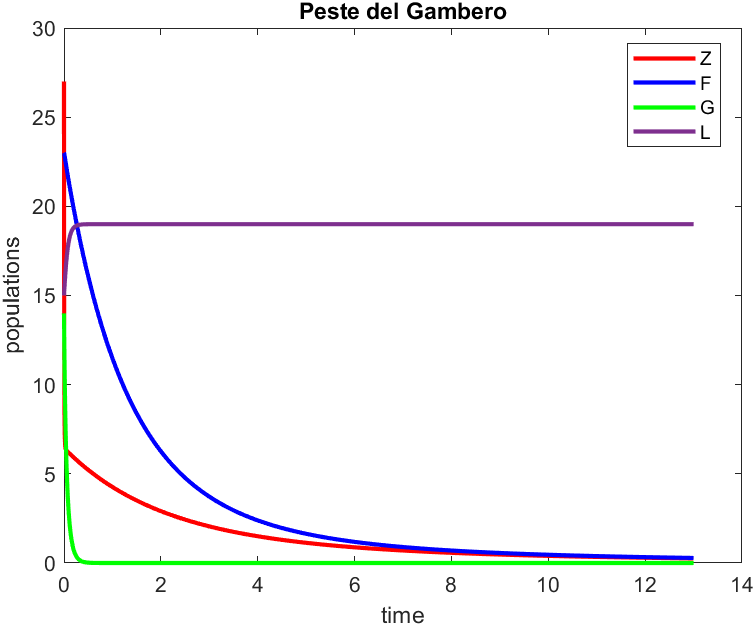
\includegraphics[width=6 cm]{grafici/E1_fasi.png} 
    \\
    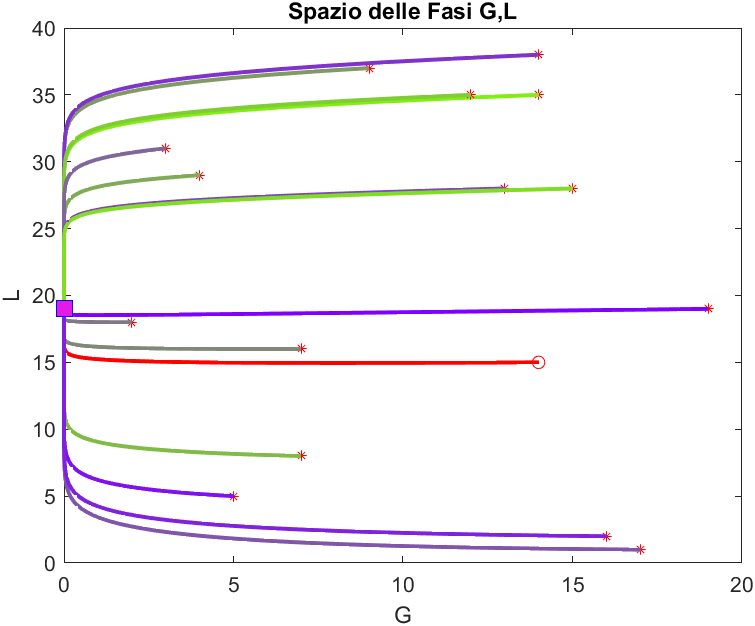
\includegraphics[width=6 cm]{grafici/E1_ritratto.png}
    \captionof{figure}{Popolazioni nel tempo e ritratto di fase per l'equlibrio $E_1$}
    \label{fig}
\end{minipage}

\vspace{1 cm}

\deftitle{Equilibrio $E_2$}

\begin{minipage}{0.2\textwidth}


$\begin{cases}
	c_1=25\\
	m_1=25\\
	\gamma_2=0.0075\\
	\gamma_1=0.007\\
	a_3=4\\
	c_2=30\\
	\lambda=0.005\\ %E1 Stabile
	a_1=0.05\\
	a_2=1\\
	m_2=1\\
	b_1=19\\
	b_2=7\\
	m_3=1\\
	m_4=1\\
	
\end{cases}$ \\
\end{minipage}
\begin{minipage}{0.7\textwidth}
    \centering
    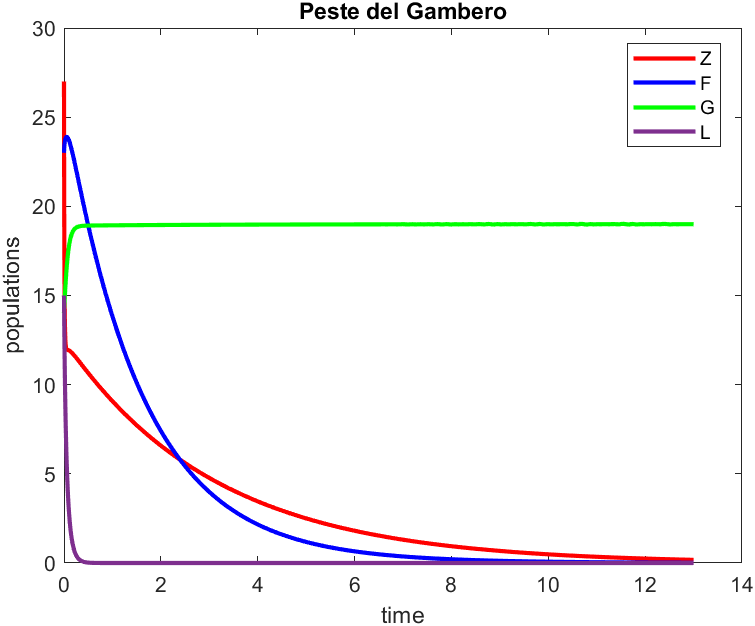
\includegraphics[width=6 cm]{grafici/E2_fasi.png} 
    \\
    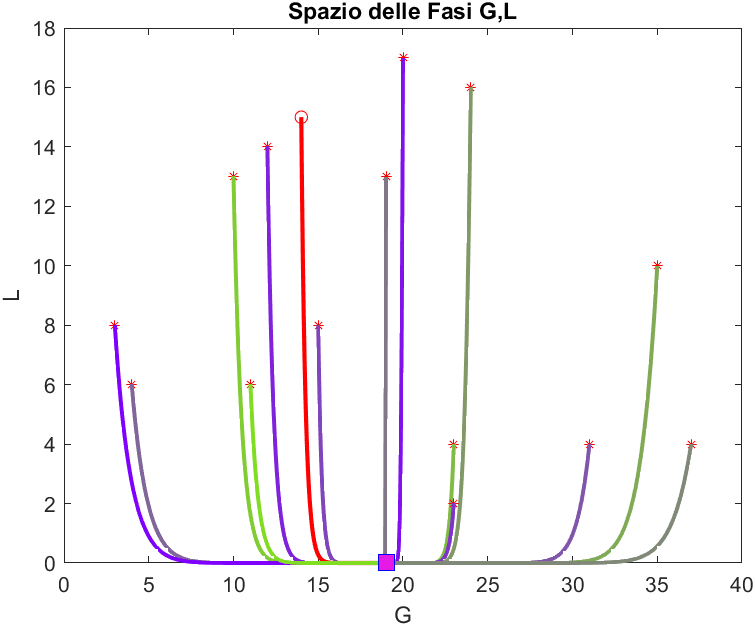
\includegraphics[width=6 cm]{grafici/E2_ritratto.png}
    \captionof{figure}{Popolazioni nel tempo e ritratto di fase per l'equlibrio $E_2$}
\end{minipage}

\newpage

\deftitle{Equilibrio $E_3$}

\begin{minipage}{0.2\textwidth}


$\begin{cases}
	c_1=45\\
	m_1=40 \\
	\gamma_2=0.00075\\
	\gamma_1=0.0007\\
	a_3=4\\
	c_2=3\\
	\lambda=0.005\\ %E3 Stabile
	a_1=0.2\\
	a_2=0.2\\
	m_2=15\\
	b_1=19\\
	b_2=19\\
	m_3=1\\
	m_4=1\\
\end{cases}$ 
\end{minipage}
\begin{minipage}{0.7\textwidth}
    \centering
    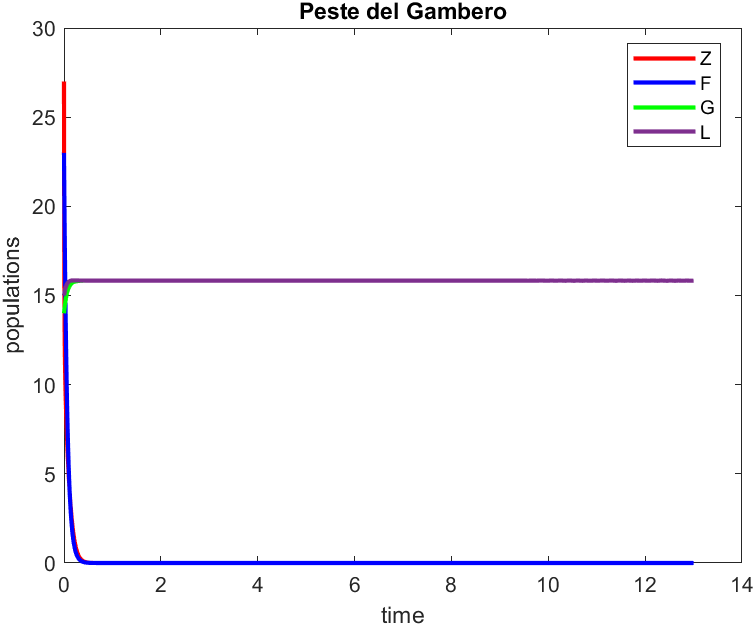
\includegraphics[width=6 cm]{grafici/E3_fasi.png} 
    \\
    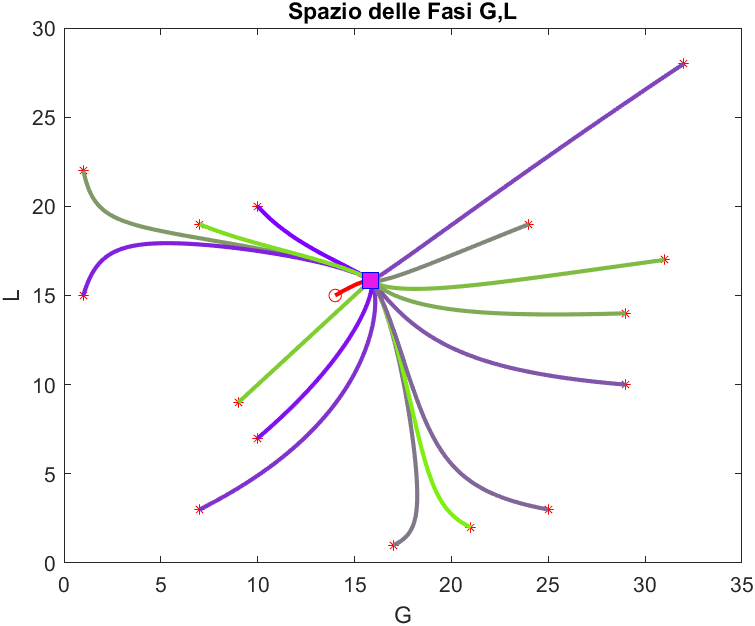
\includegraphics[width=6 cm]{grafici/E3_ritratto.png}
    \captionof{figure}{Popolazioni nel tempo e ritratto di fase per l'equlibrio $E_3$}
\end{minipage}

\vspace{1 cm}

\deftitle{Equilibrio $E_4$}

\begin{minipage}{0.2\textwidth}

$\begin{cases}
	c_1=250\\
	m_1=2\\
	\gamma_2=0.0072\\
	\gamma_1=0.0075\\
	a_3=4\\
	c_2=30\\
	\lambda=0.5\\ %E4 Stabile
	a_1=0.5\\
	a_2=1\\
	m_2=1\\
	b_1=19\\
	b_2=7\\
	m_3=1\\
	m_4=1\\  
\end{cases}$ 
\end{minipage}
\begin{minipage}{0.7\textwidth}
    \centering
    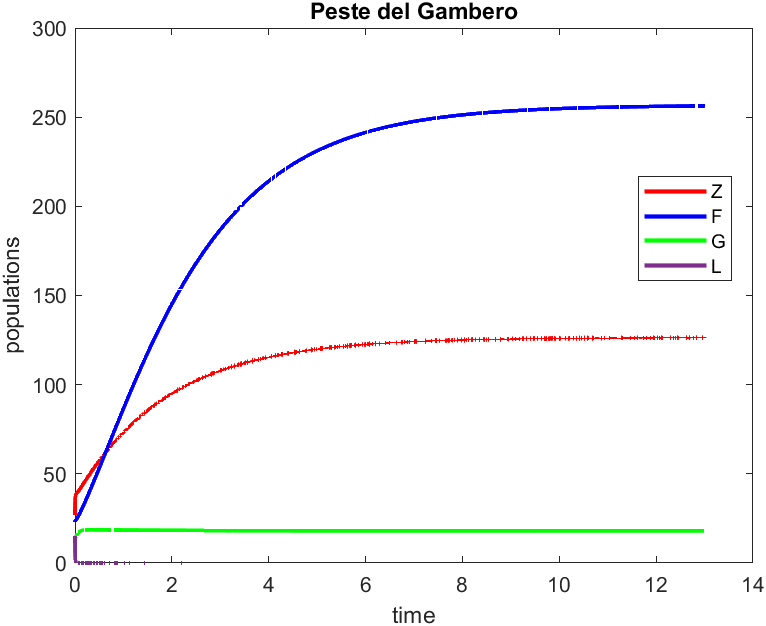
\includegraphics[width=6 cm]{grafici/E4_fasi.png} 
    \\
    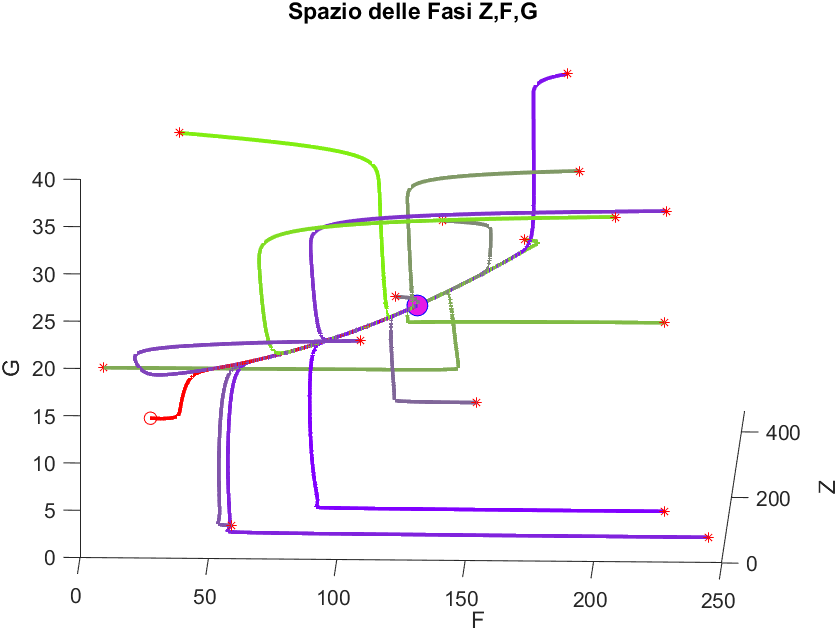
\includegraphics[width=6 cm]{grafici/E4_ritratto.png}
    \captionof{figure}{Popolazioni nel tempo e ritratto di fase per l'equlibrio $E_4$}
\end{minipage}

\newpage

\deftitle{Equilibrio $E_5$}

\begin{minipage}{0.2\textwidth}


$\begin{cases}
	c_1=25\\
	m_1=2\\
	\gamma_2=0.0075\\
	\gamma_1=0.007\\
	a_3=4\\
	c_2=30\\
	\lambda=0.005\\ %E5 Stabile
	a_1=1\\
	a_2=0.5\\
	m_2=0.64\\
	b_1=7\\
	b_2=19\\
	m_3=1\\
	m_4=1\\
\end{cases}$ 
\end{minipage}
\begin{minipage}{0.7\textwidth}
    \centering
    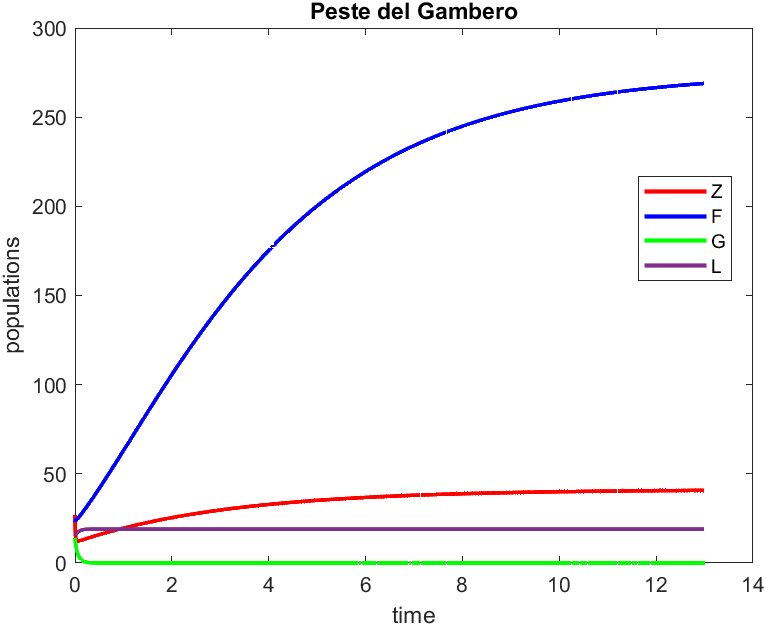
\includegraphics[width=6 cm]{grafici/E5_fasi.png} 
    \\
    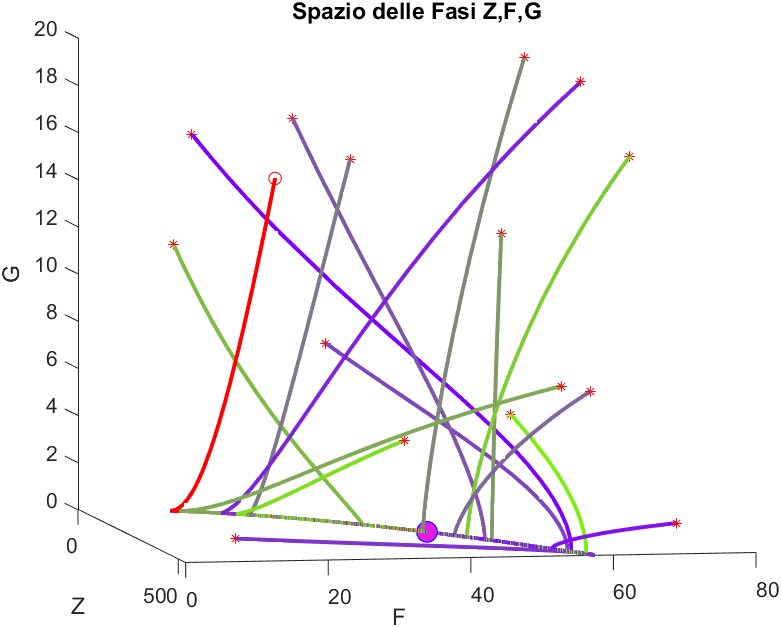
\includegraphics[width=6 cm]{grafici/E5_ritratto.png}
    \captionof{figure}{Popolazioni nel tempo e ritratto di fase per l'equlibrio $E_5$}
\end{minipage}

\vspace{1 cm}

\deftitle{Equilibrio $E_6$}

\begin{minipage}{0.2\textwidth}
    $\begin{cases}
	c_1=150\\
	m_1=6\\
	\gamma_2=0.0075\\
	\gamma_1=0.007\\
	a_3=4\\
	c_2=45\\
	\lambda=0.5\\ %E6 Stabile
	a_1=0.2\\
	a_2=0.2\\
	m_2=7\\
	b_1=19\\
	b_2=19\\
	m_3=1\\
	m_4=1\\ 
\end{cases}$
\end{minipage}
\begin{minipage}{0.7\textwidth}
    \centering
    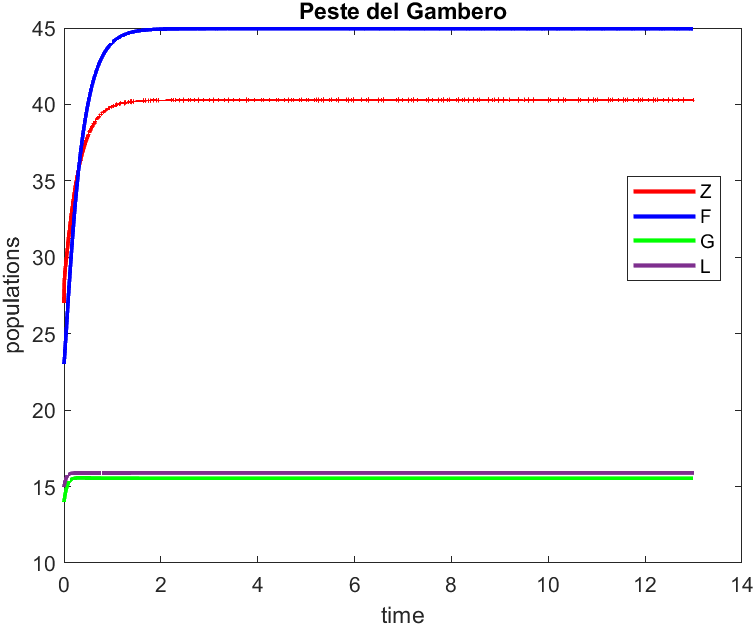
\includegraphics[width=6 cm]{grafici/E6_fasi.png} 
    \\
    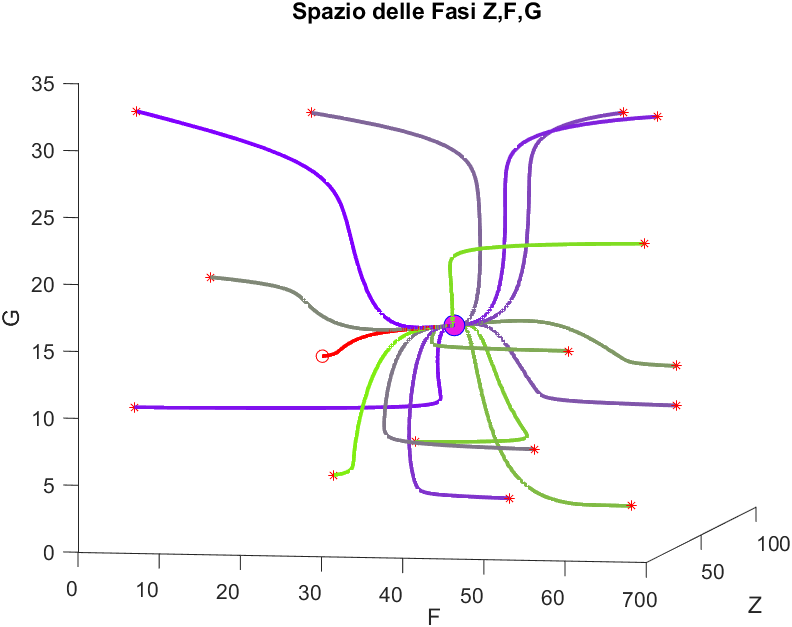
\includegraphics[width=6 cm]{grafici/E6_ritratto.png}
    \captionof{figure}{Popolazioni nel tempo e ritratto di fase per l'equlibrio $E_6$}
\end{minipage}

\newpage
\subsection{Bistabilità}
È stato anche possibile individuare alcuni casi di bistabilità: per le coppie di equilibri $(E_4,E_5)$,$(E_2,E_5)$ ed $(E_1,E_2)$.

\smallskip
\[E_4,E_5:\begin{cases}
	c_1=250\\
	m:1=2\\
	\gamma_2=0.0072\\
	\gamma_1=0.0075\\
	a_3=4\\
	c_2=30\\
	\lambda=0.5\\ %Bistabilità E4 E5
	a_1=7\\
	a_2=7\\
	m_2=1\\
	b_1=19\\
	b_2=19\\
	m_3=1\\
	m_4=1\\
\end{cases}E_2,E_5:\begin{cases}
	c_1=250\\
	m_1=20\\
	\gamma_2=0.0072\\
	\gamma_1=0.0075\\
	a_3=41\\
	c_2=35\\
	\lambda=0.0005\\ %bistabilita E2,E5
	a_1=2\\
	a_2=5\\
	m_2=1\\
	b_1=17\\
	b_2=11\\
	m_3=1\\
	m_4=1\\
\end{cases}E_1,E_2:\begin{cases}
c_1=45\\
 m_1=40\\
 \gamma_2=0.00075\\
 \gamma_1=0.0007\\
 a_3=4\\
 c_2=3\\
 \lambda=0.005\\ %bistabilita E1,E2
 a_1=3\\
 a_2=3\\
 m_2=15\\
 b_1=19\\
 b_2=19\\
 m_3=1\\
 m_4=1\\
\end{cases}\]
\begin{figure}[h!]
    \centering
    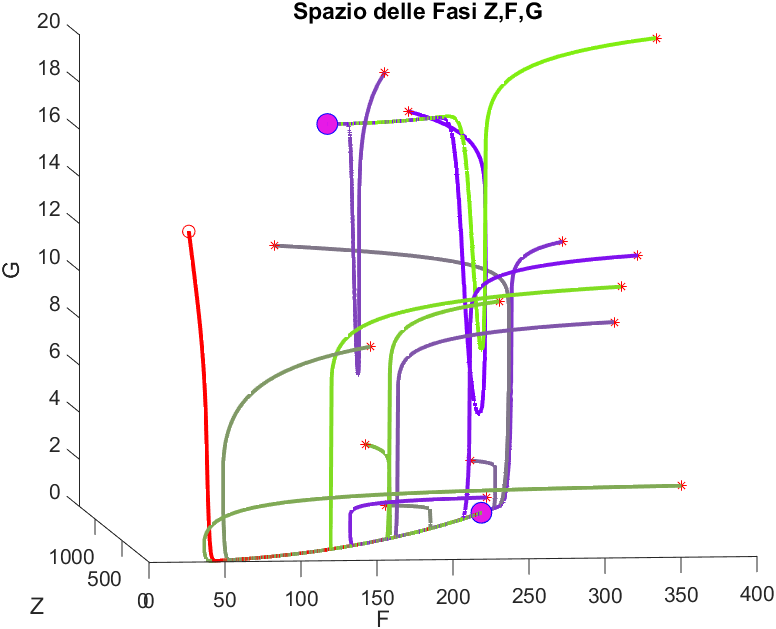
\includegraphics[width=7cm]{grafici/bistab.png}
    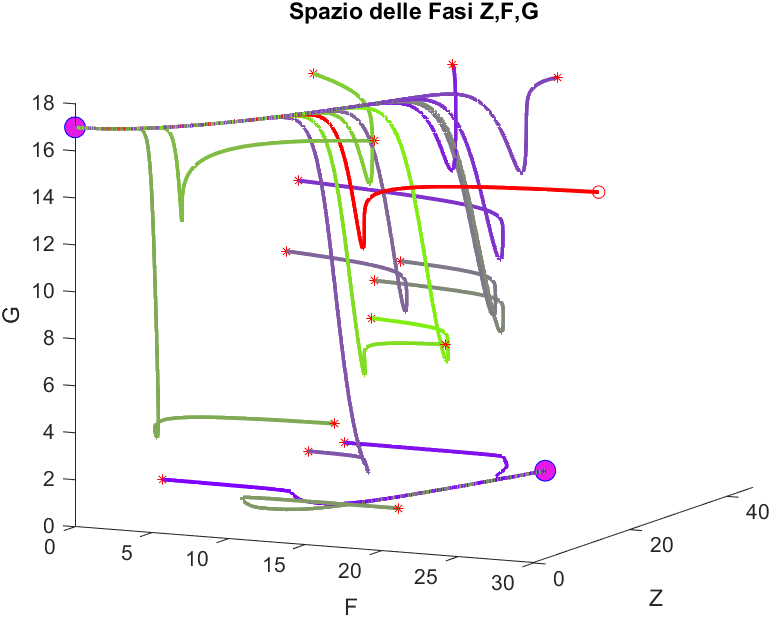
\includegraphics[width=7cm]{grafici/bistab2.png}
    \\
    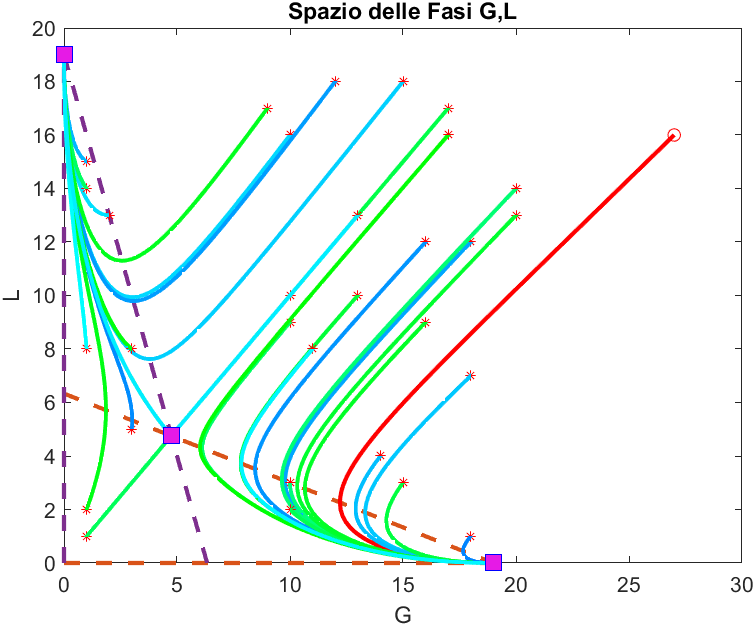
\includegraphics[width=7cm]{grafici/bistab3.png}
    \caption{I tre ritratti di fase ($(E_4,E_5)$, $(E_2,E_5)$) ed $(E_1,E_2)$ nel caso di bistabilità, notare come nella bistabilità di $E_1,E_2$, l'equilibrio $E_3$ che si trova sull'intersezione delle isoclinee di crescita zero (rette tratteggiate), separi i due bacini d'attrazzione.}
    \label{fig:E7}
\end{figure}

\newpage

\subsection{Biforcazioni di Hopf}
Dalle simulazioni numeriche, abbiamo trovato dei valori dei parametri per cui le popolazioni convergevano in maniera oscillatoria all'equilibrio $E_4$, si veda \ref{tab_hopf} per i valori. 
Analizzando inoltre il ritratto di fase nello spazio $Z,F,G$, sembrerebbe proprio che l'equilibrio $E_4$ abbia tutta la faccia di un pozzo a spirale, o il suo analogo in dimensione $4$.
\begin{table}[h!]
\centering
 \begin{tabular}{|c|c|c|c|c|c|c|c|c|c|c|c|c|c|}
 \hline
  $a_1$ & $a_2$ & $a_3$ & $\lambda$ & $b_1$ & $b_2$ & $c_1$  & $c_2$ & $m_1$ & $m_2$ & $m_3$ & $m_4$ & $\gamma_1$ & $\gamma_2$\\
  \hline
  $20$ & $0.2$ & $0.2$ & $0.5$ & $40$ & $4$ & $10$ &  $10$ & $20$ & $1$ & $0.2$ & $6$ & $0.35$ & $0.07$ \\
  \hline
 \end{tabular}
 \caption{Tabella dei parametri utilizzati per la Figura \ref{hopf1}.}
 \label{tab_hopf}
\end{table}

\begin{figure}[h!]
    \centering
    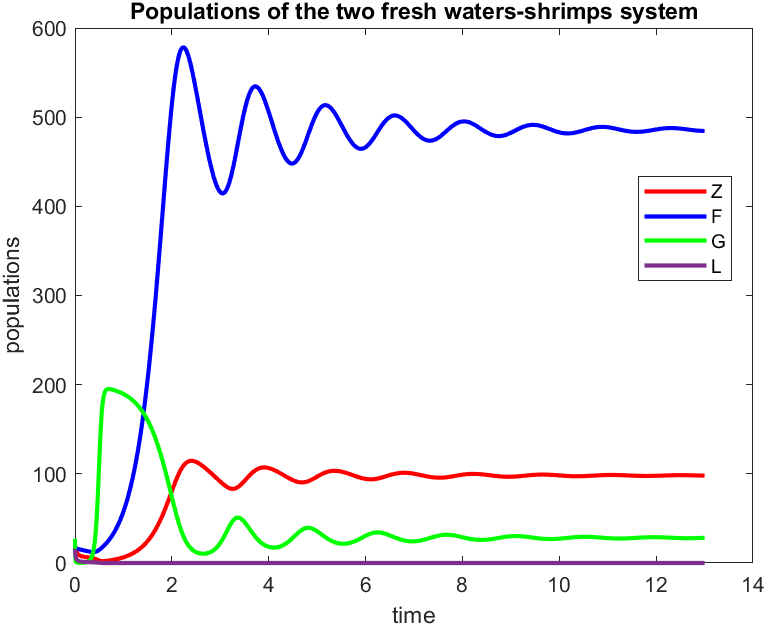
\includegraphics[width=8 cm]{grafici/hopf_prima_popolazioni.png} 
    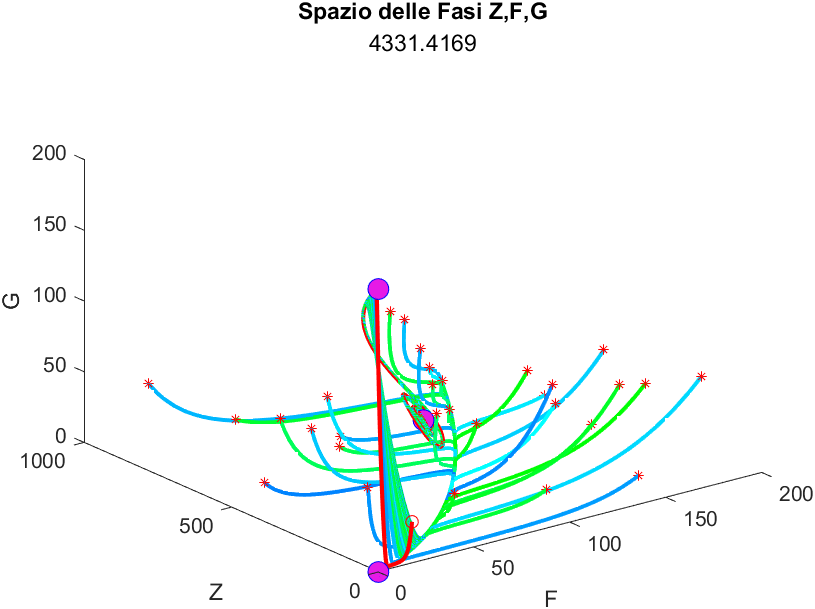
\includegraphics[width=8 cm]{grafici/hopf_prima_fasi.png}
    \captionof{figure}{Popolazioni nel tempo e ritratto di fase per l'equlibrio $E_4$ con $\gamma_1=0.35$}
    \label{hopf1}
\end{figure}

Inoltre, incrementando il rate d'infezione sui gamberi autoctoni, la stabilità di $E_4$ scompare e le traiettorie convergono verso un ciclo limite. 



\begin{figure}[h!]
    \centering
    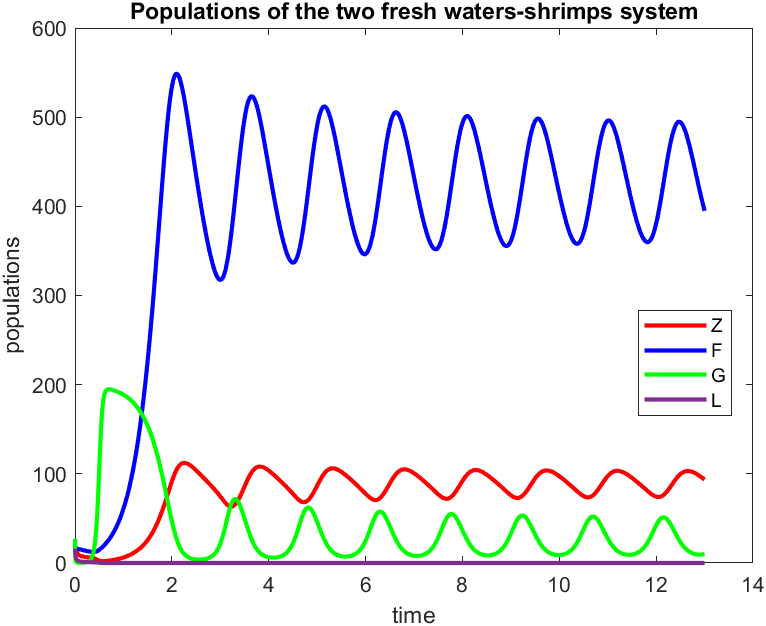
\includegraphics[width=8 cm]{grafici/hopf_dopo_popolazioni.png} 
    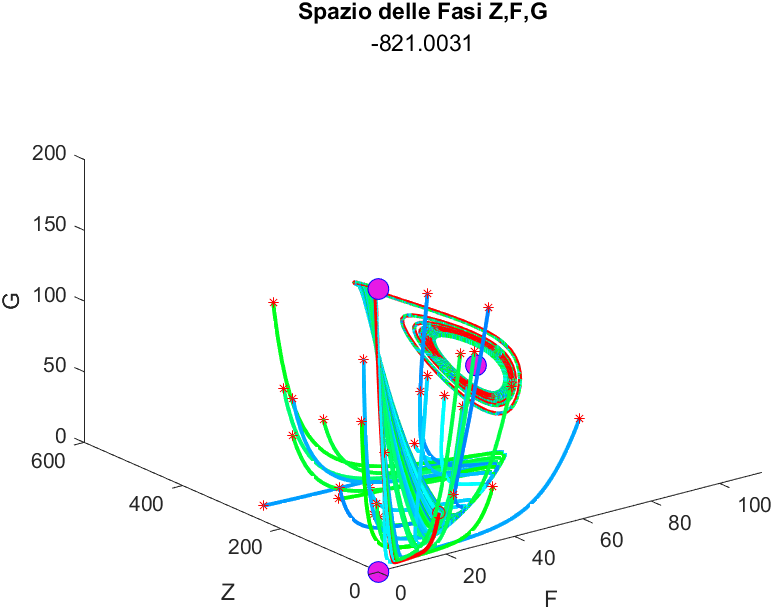
\includegraphics[width=8 cm]{grafici/hopf_dopo_fasi.png}
    \captionof{figure}{Popolazioni nel tempo e ritratto di fase per l'equlibrio $E_4$, con $\gamma_1=0.39$}
    \label{hopf2}
\end{figure}

Insomma sembrerebbe proprio che sia comparsa una biforcazione di Hopf. In effetti si può constatare che a cambiare di segno è l'ultima condizione dell'equilibrio $E4$ dovuta a Routh-Hurwitz, come si può vedere sotto ai titoli delle figure \ref{hopf1} e \ref{hopf2}. Ricordiamo che tale quantità è data da
\begin{equation}
\label{r_h_hopf}
    A_2A_1-A_0
\end{equation}
con gli appositi coefficienti del polinomio di terzo grado.

Abbiamo allora cercato quale valore di $\gamma_1$, compreso fra $0.35$ e $0.39$ annullasse \ref{r_h_hopf}. Si trova che tale valore vale circa $0.3822914034$, come si può constatare da \ref{hop3}, in effetti inserendo tale valore nelle simulazioni si vede che si è poco dopo il valore esatto di biforcazione (si è appena formato il ciclo limite, e la condizione di R-H \ref{r_h_hopf} è quasi nulla, di poco negativa).

\begin{figure}[h!]
    \centering
    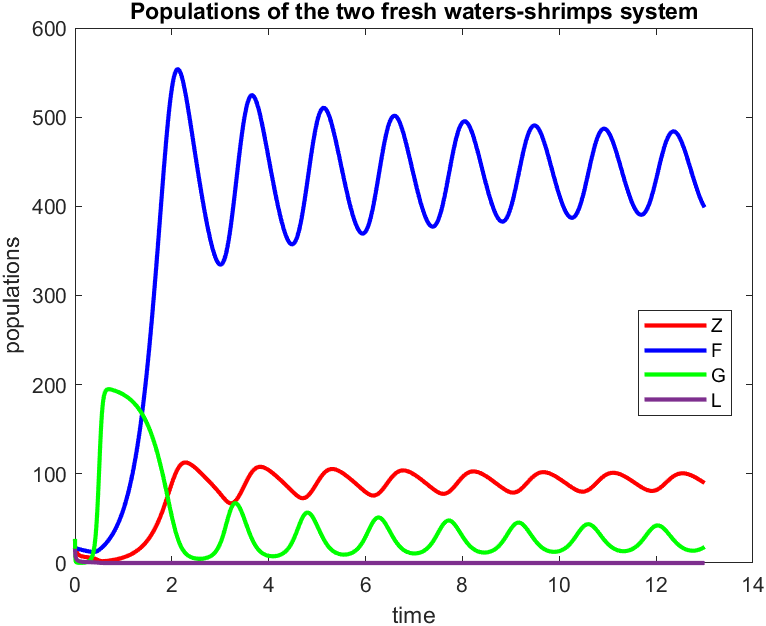
\includegraphics[width=8 cm]{grafici/hopf_valore_popolazioni.png} 
    \includegraphics[width=8 cm]{grafici/hopf_valore_fasi.png}
    \captionof{figure}{Popolazioni nel tempo e ritratto di fase per l'equlibrio $E_4$,con $\gamma_1=0.3822914034$}
    \label{hop3}
\end{figure}

\color{white} filler \color{black}

\newpage
\appendix

\section{Criterio di Routh-Hurwitz}
Consideriamo un polinomio di grado $n$ a coefficienti reali della forma
 \begin{equation*}
     p(s)=a_n s^n + a_{n-1} s^{n-1} + \cdots + a_1 s + a_0
 \end{equation*}
Diremo \textbf{matrice di Routh} del polinomio $p$ la matrice in $\mathbb{R}^{n+1,n}$ della forma
 \begin{equation*}
    \begin{bmatrix} 
        a_n & a_{n-2} & a_{n-4} & a_{n-6}  & \ldots   \\
        a_{n-1} & a_{n-3} & a_{n-5} & \ldots  \\
        b_{n-1} & b_{n-2} & \ldots & \\
        c_{n-2} & c_{n-3} & &
    \end{bmatrix}
 \end{equation*}
dove 
\begin{itemize}
    \item  $b_{n-1} = -\frac{
\begin{vmatrix}
a_n & a_{n-2} \\
a_{n-1} & a_{n-3}
\end{vmatrix}
}{a_{n-1}}$ \\
\item $b_{n-2} = -\frac{\begin{vmatrix}
a_n & a_{n-4} \\
a_{n-1} & a_{n-5}
\end{vmatrix}}{a_{n-1}}$ \\
\item $c_{n-2} = -\frac{\begin{vmatrix}
a_{n-1} & a_{n-3} \\
b_{n-1} & b_{n-2}
\end{vmatrix}}{b_{n-1}}$ 
\item  $c_{n-3} = -\frac{\begin{vmatrix}
a_{n-1} & a_{n-5} \\
b_{n-1} & b_{n-3}
\end{vmatrix}}{b_{n-1}}$ \\
\end{itemize}
 Ossia più in generale nel posto $(i,j)$ della matrice di Routh inseriamo il rapport fra il determinante della matrice $2\times 2$ ottenuta mettendo nella prima colonna, le due precedenti entrate della prima colonna della matrice di Routh (quindi gli elementi al posto $(i-1,1),(i-2,1)$, e sulla seconda colonna i due precedenti termini della colonna $j$-esima dellamatrice di Routh, ossia gli elementi di posto $(i-1,j),(i-2,j)$, e dividendo il tutto per l'elemento in posizione $(i-1,1)$ Se definiamo $R_{i,j}$ gli elementi della matrice di Routh, questo significa che la costruizione iterativa della matrice di Routh è data da
\[
R_{1,j+1}=a_{n-2j},\quad j=0,\dots, \left\lfloor \frac n 2 \right\rfloor,\qquad R_{2,k+1}=a_{n-2k-1},\quad k=0,\dots, \left\lfloor \frac {n-1} 2\right\rfloor \] 
\[
R_{1,j+1}=0,\quad j>\left\lfloor \frac n 2 \right\rfloor, \qquad R_{2,k+1}=0,\quad k>\left\lfloor \frac {n-1} 2 \right\rfloor \qquad  \] 
\[
   R_{i,j} = -\frac{
\begin{vmatrix}
R_{i-2,1}& R_{i-2,j} \\
R_{i-1,1} & R_{i-1,j}
\end{vmatrix}
}{R_{i-1,1}} \\
\]

\newpage
Passiamo all'enunciato del teorema di Routh-Hurwitz
 \begin{theo}[\deftitle{Criterio di Routh-Hurwitz}]{}
 \label{ap:A}
     Dato un polinomio a coefficienti 
      \begin{equation*}
          p(s)=a_n s^n + a_{n-1} s^{n-1} + \cdots + a_1 s + a_0, \text{ tale che } a_i \neq 0 \; \forall i = 1, \dots, n
      \end{equation*}
     le radici del polinomio $p$ sono negative se e solo se tutti i coefficienti di $p$ hanno lo stesso segno e se tutti gli elementi della prima colonna della matrice di Routh hanno lo stesso segno. In particolare, se il polinomio è monico, i coefficienti e i termini della prima colonna devono essere tutti positivi. \\
 \end{theo}
Ricordiamo allora nello specifico i criteri nel caso di polinomi monici di grado $3$ e $4$.
\begin{itemize}
\item[\balln{yellow}{$1$}] per $q(s) = s^3 + A_2 s^2 + A_1 s +A_0$ la matrice di Routh è data da
\begin{equation*}
	\begin{bmatrix} 
		1 & A_1 & 0 \\
		A_2 & A_0 & 0 \\
		\frac{(A_2 A_1 - A_0)}{A_2} & 0 & 0 \\
		A_0 & 0 & 0 \\
	\end{bmatrix}
\end{equation*}
Ricaviamo allora le seguenti condizioni per avere parte reale negativa in tutte le radici, da Routh-Hurwitz:
 \[
 \begin{cases*}
     A_i>0, \quad i=0,\dots,2 \\
     A_2 A_1 - A_0>0 \\
 \end{cases*}
 \]
\item[\balln{yellow}{$2$}]  Prendiamo un polinomio monico di grado tre $$p(s) = s^4 + A_3 s^3 + A_2 s^2 + A_1 s +A_0$$
Allora, la matrice di Routh è data da 
	\begin{equation*}
		\begin{bmatrix} 
			1 & A_2 & A_0 & 0 \\
			A_3 & A_1 & 0 & 0 \\
			\frac{A_3 A_2 - A_1}{A_3} & A_0 & 0 & 0 \\
			\frac{(A_3 A_2 - A_1)A_1 - A_3^2 A_0}{A_3 A_2 - A_1} & 0 & 0 & 0 \\
			A_0 & 0 & 0 & 0
		\end{bmatrix}
	\end{equation*}
 Ne segue che le condizioni per avere tutte le radici di parte reale negativa, date dal criterio di Routh-Hurwitz, sono
 \[
 \begin{cases*}
     A_i>0, \quad i=0,\dots,3 \\
     A_3 A_2 - A_1>0 \\
     (A_3 A_2 - A_1)A_1 - A_3^2 A_0>0
 \end{cases*}
 \]
 Ossia le stesse per un polinomio di terzo grado, a cui si aggiunge \\ $A_3>0,(A_3 A_2 - A_1)A_1 - A_3^2 A_0>0$ .
 \end{itemize}


 












%Alcune ipotesi sui parametri che si potrebbero fare per semplificare un po' il modello sono:

%\begin{itemize}[\palla]
	%\item il Gambero Louisiano risente praticamente non risente della competizione $\implies$ $a_2=0$
	%\item possiamo suppore che il rate d'infezione sia simile per i gamberi $\implies$ $\gamma_1=\gamma_2=\gamma$
	%\item fissare $c_1$ e $c_2$
%\end{itemize}
%Il modello allora sarebbe

%$$\begin{cases*}
	%\dot Z= c_1F-m_1 Z -\gamma(L+G)Z - a_3 Z^2 \\
	%\dot F= c_2 \gamma(LZ  + \lambda GZ)- m_2 F \\
	%\dot G= -\gamma_1 GZ - a_1 LG+b_1 G -m_3 G^2 \\
	%\dot L= b_2 L -m_4 L^2 
%\end{cases*}$$







\newpage

\begin{thebibliography}{10}

\bibitem[1]{mase.gov}
  {Ministero dell'ambiente e della sicurezza energetica},
  \textit{Piano di gestione nazionale del Gambero rosso della Louisiana},
  {2003},
  \url{https://www.mase.gov.it/pagina/piano-di-gestione-nazionale-del-gambero-rosso-della-louisiana}

\bibitem[2]{lifeclaw}
  {LifeClaw},
  \textit{L'importanza del gambero dolce},
  \url{https://www.lifeclaw.eu/i-gamberi-di-fiume/}

\bibitem[3]{lifeclawazioni}
  {LifeClaw},
  \textit{Le azioni},
  \url{https://www.lifeclaw.eu/il-progetto/azioni/}

\bibitem[4]{rizzato2015presenza}
  {Rizzato, Andrea},
  \textit{Presenza e caratteristiche delle popolazioni di Procambarus clarkii (Girard, 1852) nella provincia di Vicenza},
  {2015}







\bibitem[5]{strand2012monitoring}
  {Strand, David A and Jussila, Japo and Viljamaa-Dirks, Satu and Kokko, Harri and Makkonen, Jenny and Holst-Jensen, Arne and Viljugrein, Hildegunn and Vr{\aa}lstad, Trude},
  \textit{Monitoring the spore dynamics of Aphanomyces astaci in the ambient water of latent carrier crayfish},
  {(Veterinary Microbiology)},
  {vol.160},
  {pp.99--107},
  {Elsevier},
  {2012}

\bibitem[6]{makkonen2013timing} 
  {Makkonen, J and Strand, DA and Kokko, H and Vr{\aa}lstad, T and Jussila, J},
  \textit{Timing and quantifying Aphanomyces astaci sporulation from the noble crayfish suffering from the crayfish plague},
  {(Veterinary Microbiology)},
  {vol.162},
  {pp.750--755},
  {Elsevier},
  {2013}

\end{thebibliography}


\end{document}